\documentclass[12pt]{article}

\usepackage{times,fullpage,xspace,fancyhdr,url}
\usepackage[pdftex]{graphicx}
\usepackage[pdftex,
            a4paper,
            colorlinks=true,
            urlcolor=black,
            linkcolor=black,
            citecolor=black,
            bookmarksopen=false,
            bookmarksnumbered=true,
            pdfstartview=FitH]{hyperref}

\usepackage{graphicx}
\usepackage{xspace,color}
\pdfcompresslevel=9
\newcommand{\leaguename}{RoboCup Standard Platform League (NAO) }
\hypersetup{
 pdftitle={\leaguename Rule Book},
 pdfauthor={Technical Committee},
}
\usepackage[latin1]{inputenc}
\usepackage{amsmath}

% comment 'disable' in to disable all the todo notes :)
\usepackage
[
%disable
]{todonotes}

\sloppy
\newcommand{\ie}{\mbox{i.\,e.}\xspace}
\newcommand{\eg}{\mbox{e.\,g.}\xspace}
\newcommand{\cf}{\mbox{cf.}\xspace}
\newcommand{\comment}[1]{\marginpar{\pdfannot width 4in height .5in depth 8pt {/Subtype /Text /Contents (#1)}}}
\newcommand{\inparagraph}[1]{\paragraph{#1\hspace{-1em} }}


% some colors
\definecolor{orange}{rgb}{1,0.5,0}
\definecolor{red}{rgb}{1,0,0}
\definecolor{green}{rgb}{0,1,0}


\title{\leaguename Rule Book}
\author{RoboCup Technical Committee}
\date{(2014 rules, as of \today)}

\setlength{\parindent}{0pt}
\setlength{\parskip}{12pt plus 6pt minus 3 pt}
\setcounter{tocdepth}{1}
\widowpenalty=10000
\clubpenalty=10000

\pagestyle{fancy}
\lhead{}
\chead{}
\rhead{}
\lfoot{}
\cfoot{}
\rfoot{}

\renewcommand{\headrulewidth}{0.4pt}
\renewcommand{\footrulewidth}{0.4pt}

\newcommand{\TotalWidth}{7.4~m\xspace}
\newcommand{\TotalLength}{10.4~m\xspace }
\newcommand{\KickOffAutoTime}{45 seconds\xspace}

% needed to align an image and text correctly side by side
\newcommand{\imagebox}[1]{\raisebox{2ex}{\raisebox{-\height}{#1}}}

\begin{document}

\maketitle

\begin{center}
Questions or comments on these rules should be mailed to \url{rc-spl-tc@lists.robocup.org}.
\end{center}

\vfill

\tableofcontents
\setcounter{tocdepth}{3}

\thispagestyle{fancy}

\clearpage

\cfoot{\thepage}
\setcounter{page}{1}

\section{Setup of the Environment}

\subsection{Field Construction}
\label{sec:field_dim}

The soccer field is built on a total carpet area of length \TotalLength and width \TotalWidth. The dimensions of the soccer field are shown in Figure~\ref{fig:field_dim}. The construction and placement of the goals is depicted in Figure~\ref{fig:goal_dimensions} and Figure~\ref{fig:goal_appearance}.

\begin{figure}[b!]
\centerline{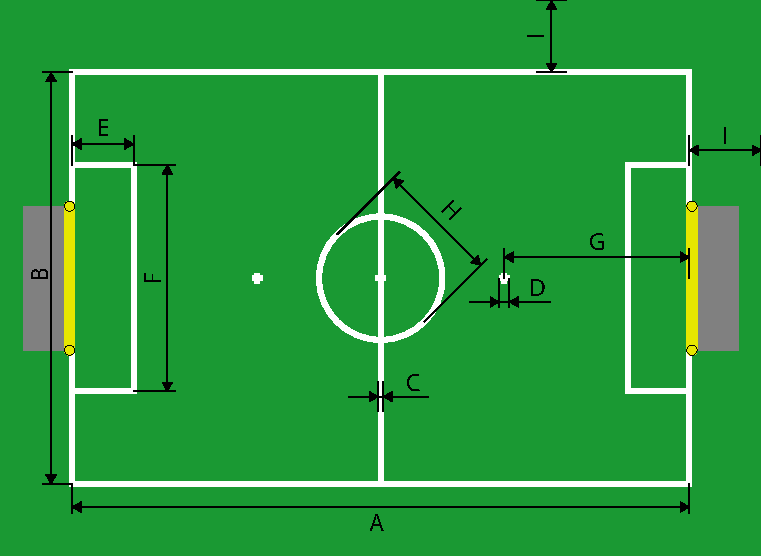
\includegraphics[width=\columnwidth]{figs/fieldDimensions2013.pdf}}
\vspace{1ex}
\begin{tabular}{| l | l | l |}
ID & Description & Length (in mm) \\
\hline
A & Field length & 9000 \\
\hline
B & Field width & 6000 \\
\hline
C & Line width & 50 \\ 
\hline
D & Penalty mark size & 100 \\ 
\hline
 &  &  \\
\end{tabular}
\begin{tabular}{|l|l|l|}
ID & Description & Length (in mm) \\
\hline
E & Penalty area length & 600 \\
\hline
F & Penalty area width & 2200 \\
\hline
G & Penalty mark distance & 1300 \\ 
\hline
H & Center circle diameter & 1500 \\
\hline
I & Border strip width & 700 \\
\end{tabular}
\caption{Schematic diagram of the soccer field (not to scale) and corresponding dimensions in mm.  Note that measurements on this diagram are made to the center of lines.} \label{fig:field_dim}
\end{figure}


\begin{figure}[t!]
\begin{center}
\leavevmode
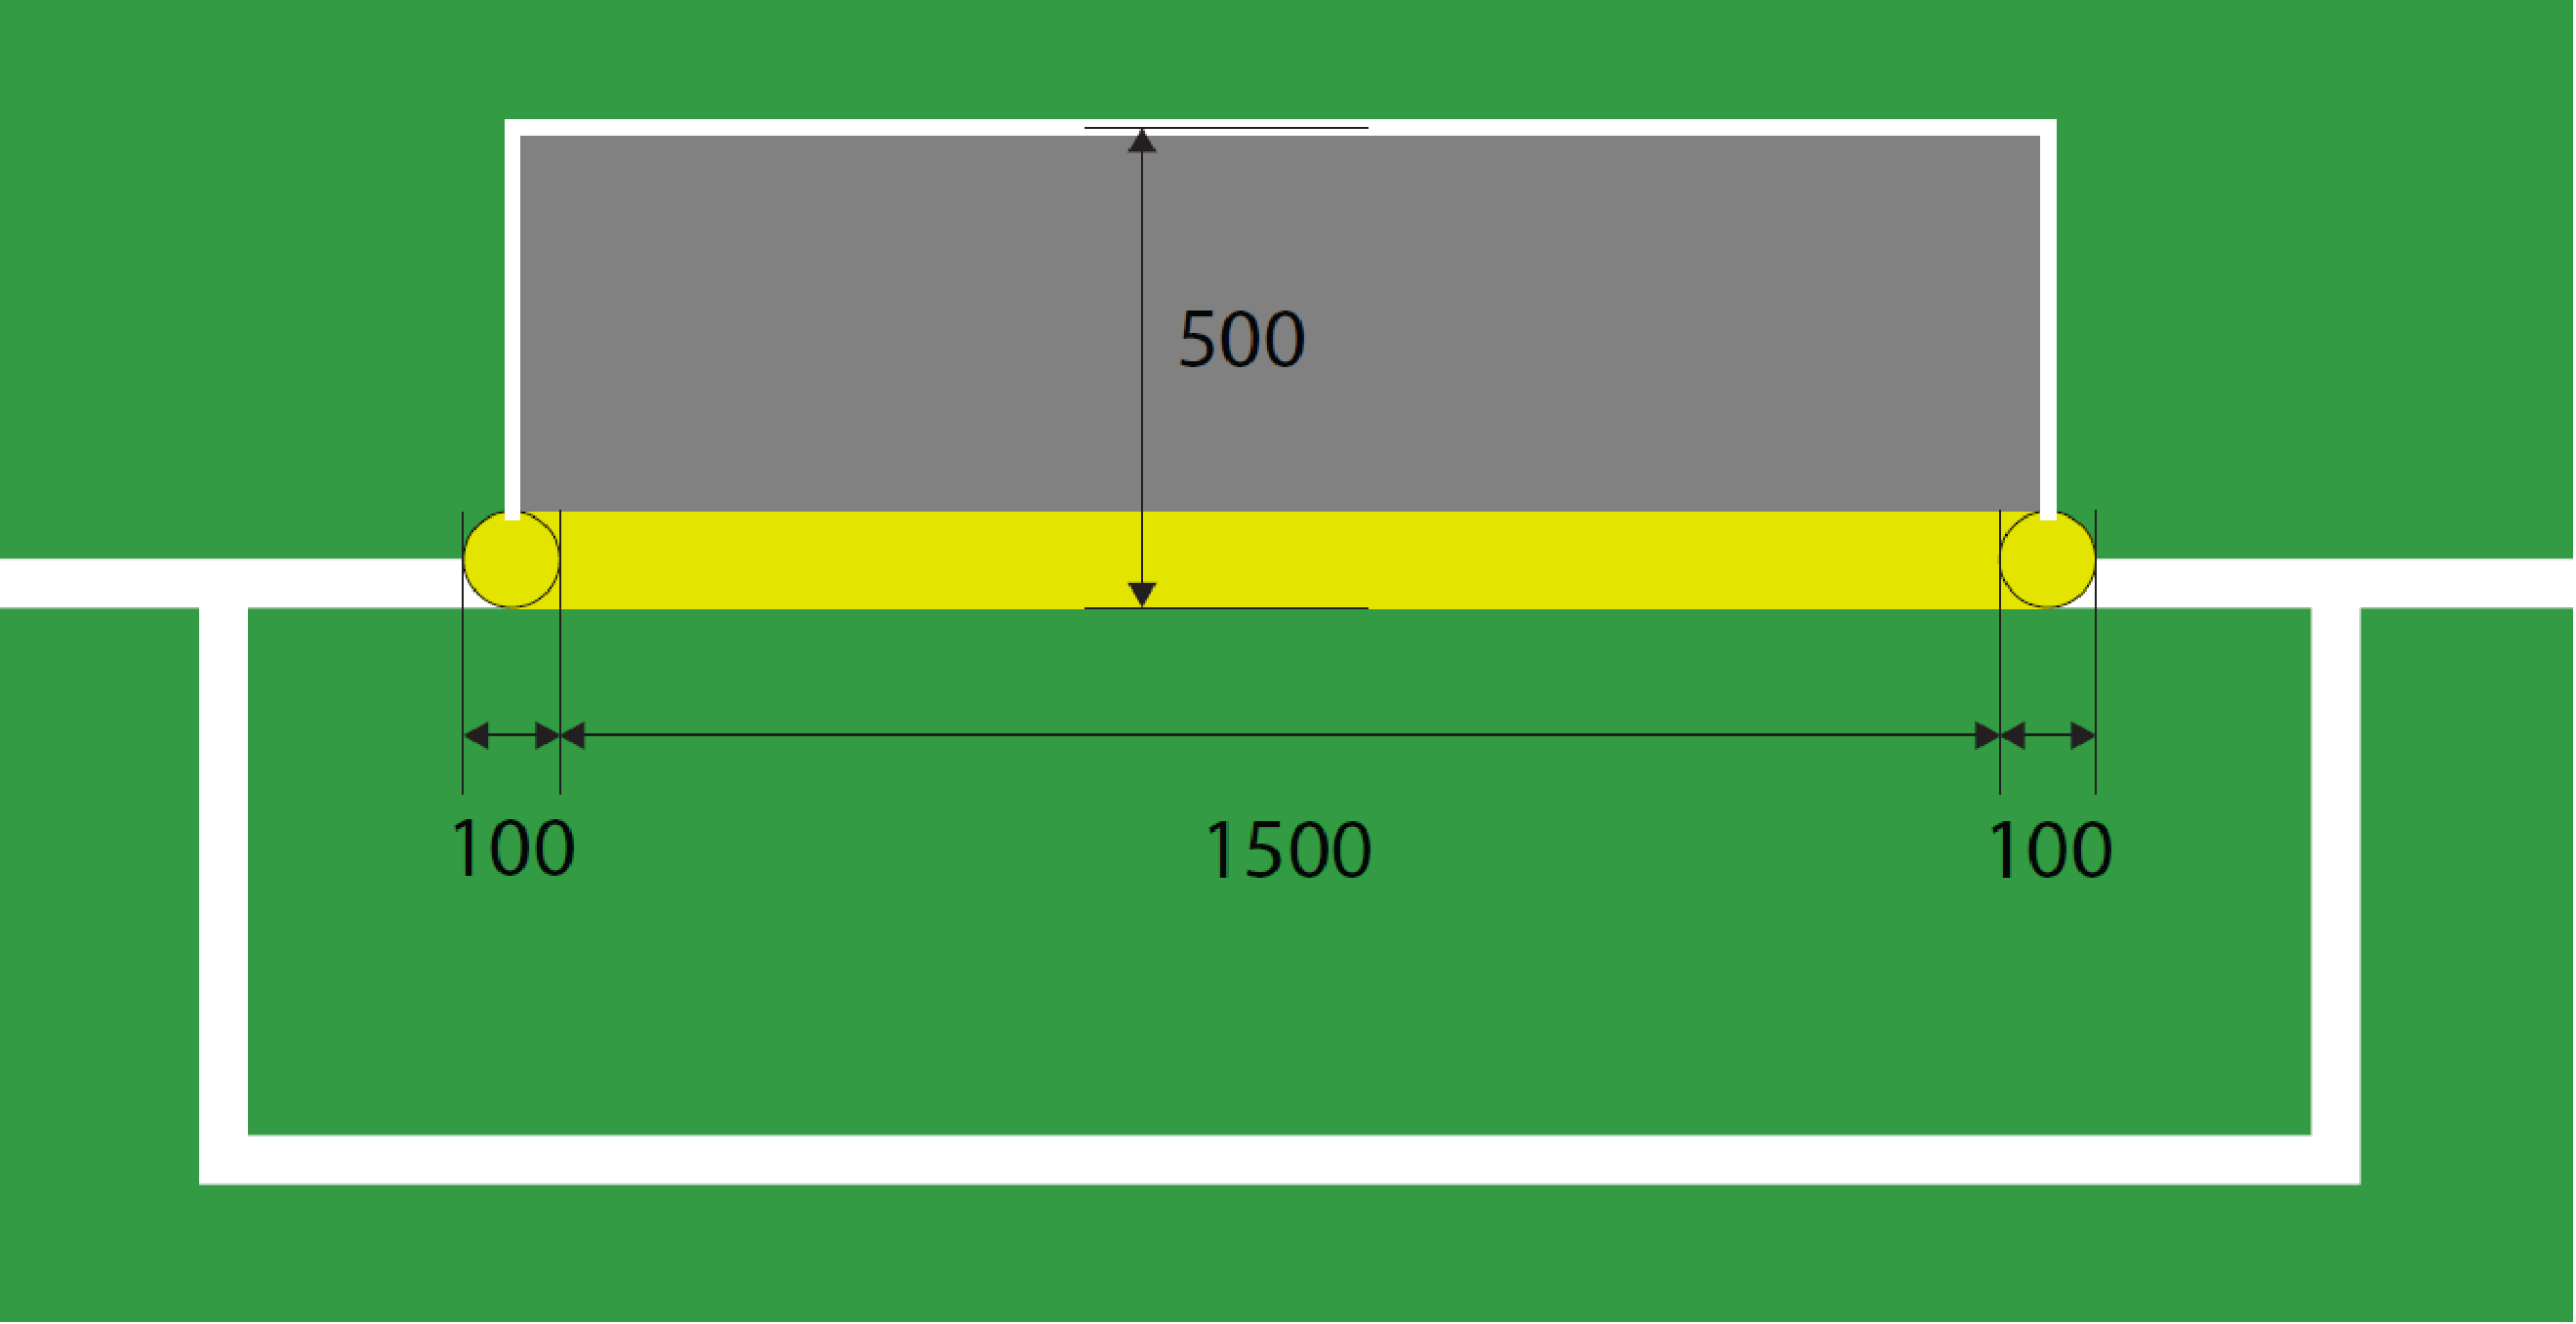
\includegraphics[width=1\columnwidth]{figs/goalDimensions.pdf}
\caption{Dimensions of the goal (in mm), viewed from above, and its placement on the field.}
\label{fig:goal_dimensions}
\end{center}
\end{figure}

\begin{figure}[h!]
\begin{center}
\leavevmode
\begin{minipage}[t]{0.49\columnwidth}
\imagebox{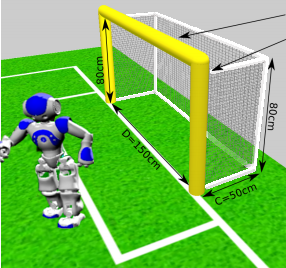
\includegraphics[width=1\columnwidth]{figs/goalDimensions3D.png}}%
\end{minipage}
\begin{minipage}[t]{0.49\columnwidth}
The goalposts and crossbar are made from 3 yellow cylinders with a diameter of 10 cm. 
The net:
\begin{itemize}
\item has a height of 80 cm
\item is of white, grey or black color
\item is tightly supported via the support structure, in a way to minimize interference with the goal keeper
\item has a weave with holes smaller than the ball diameter.
\end{itemize}
\end{minipage}
\caption{Appearance and dimensions of the goals.}
\label{fig:goal_appearance}
\end{center}
\end{figure}
The support structure for the net shall be made with small white bars or cylinders as shown in Figure \ref{fig:goal_appearance}.

\subsection{Throw-in Lines}
\label{sec:field_lines}

In addition to the visible lines, there are two invisible lines only relevant to the throw-in procedure (see Section \ref{sec:throw_in}), but not relevant to the construction of the field. These two throw-in lines are 400 mm away from the sidelines and run parallel to them inside the playing area.  Each throw-in line is 7 m long.

The throw in lines will be marked (as dots at the end of the throw in lines and short dashes along the line) by the technical committee at the start of competition with a felt-tip pen --- these lines are intended to stay invisible to robots but provide a guide to referees.

\subsection{Field Colors}

The colors of the soccer field are shown in Figure~\ref{fig:field_color}. All items on the RoboCup field are color-coded:

\begin{itemize}

\item The field (carpet) itself is green (color is not specified, but it should not be too dark).

\item The lines on the field are white.

\item Goals~(\cf Figure~\ref{fig:goal_appearance}). The posts and top cross bar of both goals are yellow (RAL 1018). The net is white, grey, or black.  The support structure for the net is white.

\end{itemize}

\begin{figure}[t]
\centerline{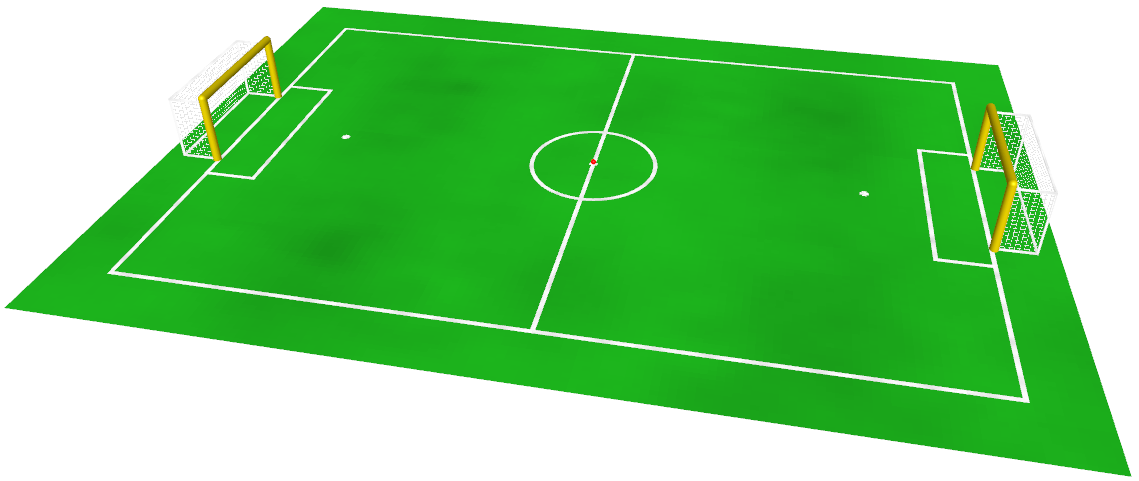
\includegraphics[width=\columnwidth]{figs/emptyfield_2014.png}}
\caption{Field colors and layout.}
\label{fig:field_color}
\end{figure}

\subsection{Lighting Conditions}

The lighting conditions depend on the actual competition site. Only ceiling lights may be used.

\subsection{Venue Setup}
\label{sec:boundaries}
Fields may be located close to one another.  Barriers will not necessarily be constructed between adjacent fields to block the robots from seeing other fields, goals, or balls.  However, barriers will be constructed to block sight between any fields that are not located at least three meters apart.  Hence, for each side of a field that is adjacent to another field, either barriers will separate the fields or at least three meters will be between the carpet of adjacent fields.

\subsection{Ball}
\label{sec:ball}

The official ball will be a Mylec orange street hockey ball. They are 65 mm in diameter and weigh 55 grams. These are the \emph{shiny} balls and are \emph{not} gel-filled.  They are no-bounce warm weather (60 to 75 degrees Fahrenheit) hockey balls.  These balls are available at a few locations:
\begin{itemize}
\item \url{http://www.amazon.com/Mylec-Weather-Bounce-Hockey-Orange/dp/B002LBDA30/ref=sr\_1\_18?ie=UTF8\&s=sporting-goods\&qid=1259775748\&sr=8-18}
\item \url{http://www.puckshop.com/mylec-orange-warm-weather-ball.html}
\end{itemize}


\newpage


\section{Robot Players}
\label{sec:robot_players}
A match is played by two teams, each consisting of not more than \textbf{5} players and a coaching robot. At most one player may be designated as \emph{goalkeeper}, the others are all \emph{field players}.

\subsection{Hardware}
\label{sec:hardware}
All teams must use NAO humanoid robots manufactured by Aldebaran Robotics. Absolutely no modifications or additions to the robot hardware are allowed. No additional hardware is permitted including off-board sensing or processing systems. Additional sensors besides those originally installed on the robots are likewise not allowed. The only exceptions are:

\begin{itemize}

\item Attaching player numbers to the heads and/or legs of the robots.  These numbers should be black with a white background, and should correspond to the number on the robot's jersey.

\item Adding black and white sponsor or team logos to the upper legs of the robots (\cf Figure~\ref{fig:sponsor}). These logos must be at least 50\% white by area.

\item Adding small black and white stickers to the torso of the robots stating the name of the robot, the name of the team, or similar information. These stickers must be at least 50\% white by area.

\item Setting the passive wrist joints to a fixed position either with glue or a transparent or white duct tape.

\item Protecting the fingers with white finger protectors provided by Aldebaran or with transparent or white duct tape.

\item Fixing the location of the upper camera using a bit of glue. \todo{Katie: I sent an email to Aldebaran, and am waiting on a reply to ensure that they are ok with this rule.}

\item Use of alternate memory sticks in replacement of the Aldebaran supplied memory sticks.

\end{itemize}

A computer will be provided by the event organizers for the purpose of sending GameController messages to the robots.

\subsection{Goal Keeper}
\label{sec:goal_keeper}

The goal keeper is allowed to touch the ball with its arms/hands only while it is within its own penalty area. It always has the jersey number ``1''.

\subsection{Field Players}
\label{sec:field_players}

Only one field player may enter their own penalty area at any given time. The four field players have the jersey numbers ``2'', ``3'', ``4'' and ``5''.

\subsection{Coaching Robot}
\label{sec:coaching_robot}

The purpose of the coaching robot is to observe the game from an external position and to give tactical and strategic advice to its team's field players. This is realized by sending messages via a dedicated GameController interface (\cf Section \ref{sec:wireless}). A coach is not directly connected to its teammates and should not serve as a remote controller or external vision system.

The coaching robot is not placed on the field but on the table that is used for the GameController computer. The coaching robot may either sit on the table or in a seat. For safety reasons, it is not allowed to move (except its head and arms --- see \cf Section \ref{sec:coach_motion}) or to enter a pose different from ordinary seating as depicted in Fig. \ref{fig:coaches}.  Seats will not be provided by the organizers, but teams may bring their own seats or small platforms that have a maximum height of the seating surface of 15 cm. Except for a backrest that is not higher than the sitting robot, no additional elements such as flags are allowed to be attached to the seats. The positions of the seats are not specified in detail and might differ from field to field. However, at each field there will be marked coaching zones (one at each side of the GameController computer) in which the coaching robots can be placed.

\begin{figure}[t]
\centerline{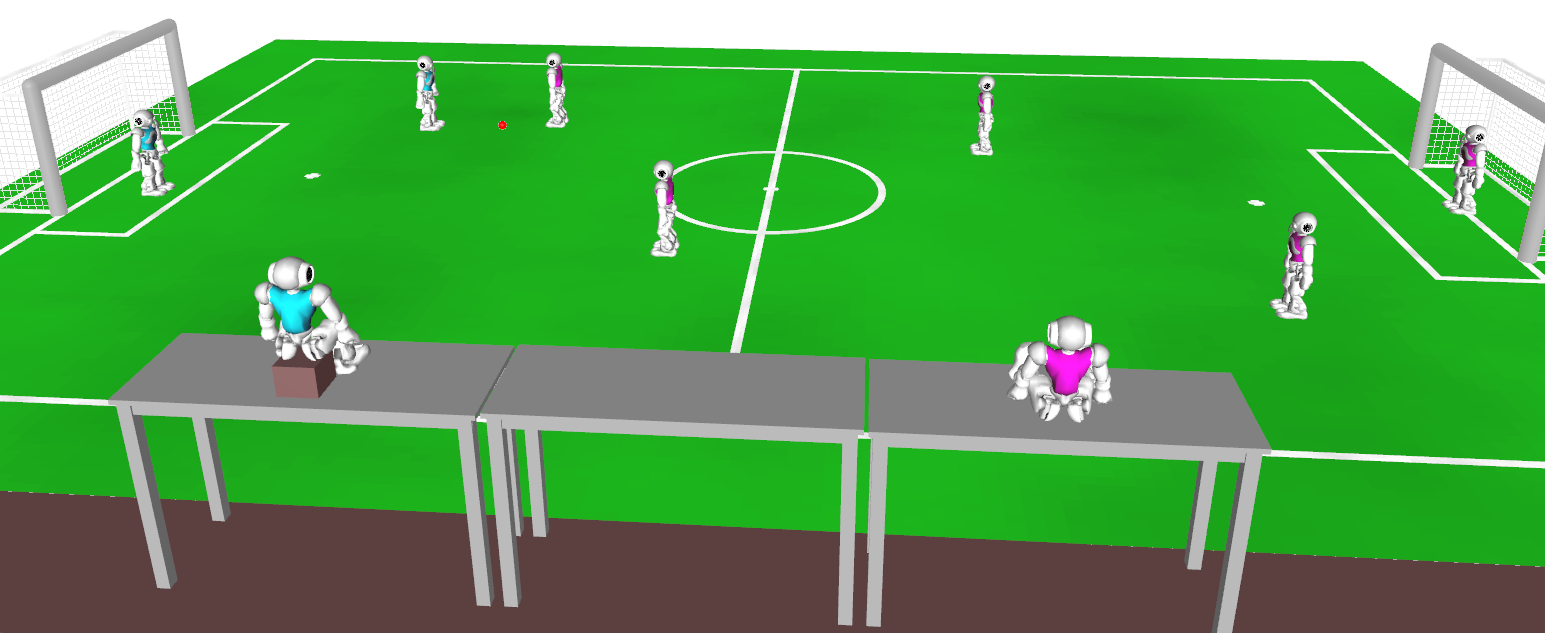
\includegraphics[width=\columnwidth]{figs/coaching-robots}}
\caption{Two coaching robots observing a game. The left robot is sitting on a seating platform. The right robot sits on the table.}
\label{fig:coaches}
\end{figure}
 

\subsection{Team Markers}
\label{sec:team_markers}

Robots use colored jersey shirts as team markers. The official jersey shirt colors are cyan and magenta (referred to as blue and red throughout this document).  Each jersey shirt has a player number(1-5) printed on it in white text.  The team markers are worn as shown in Figure~\ref{fig:nao_markers}.

Teams may use jerseys purchased at RoboCup 2013 or they may order jerseys from the league (these jerseys will be as similar as possible to the ones used at RoboCup 2013).  Teams may not use any other jersey and teams are required to have jerseys.  Information regarding purchasing jerseys will be sent out to all teams.

\begin{figure}
  \centerline{\begin{tabular}{lll}
      a) & b) & c) \\
      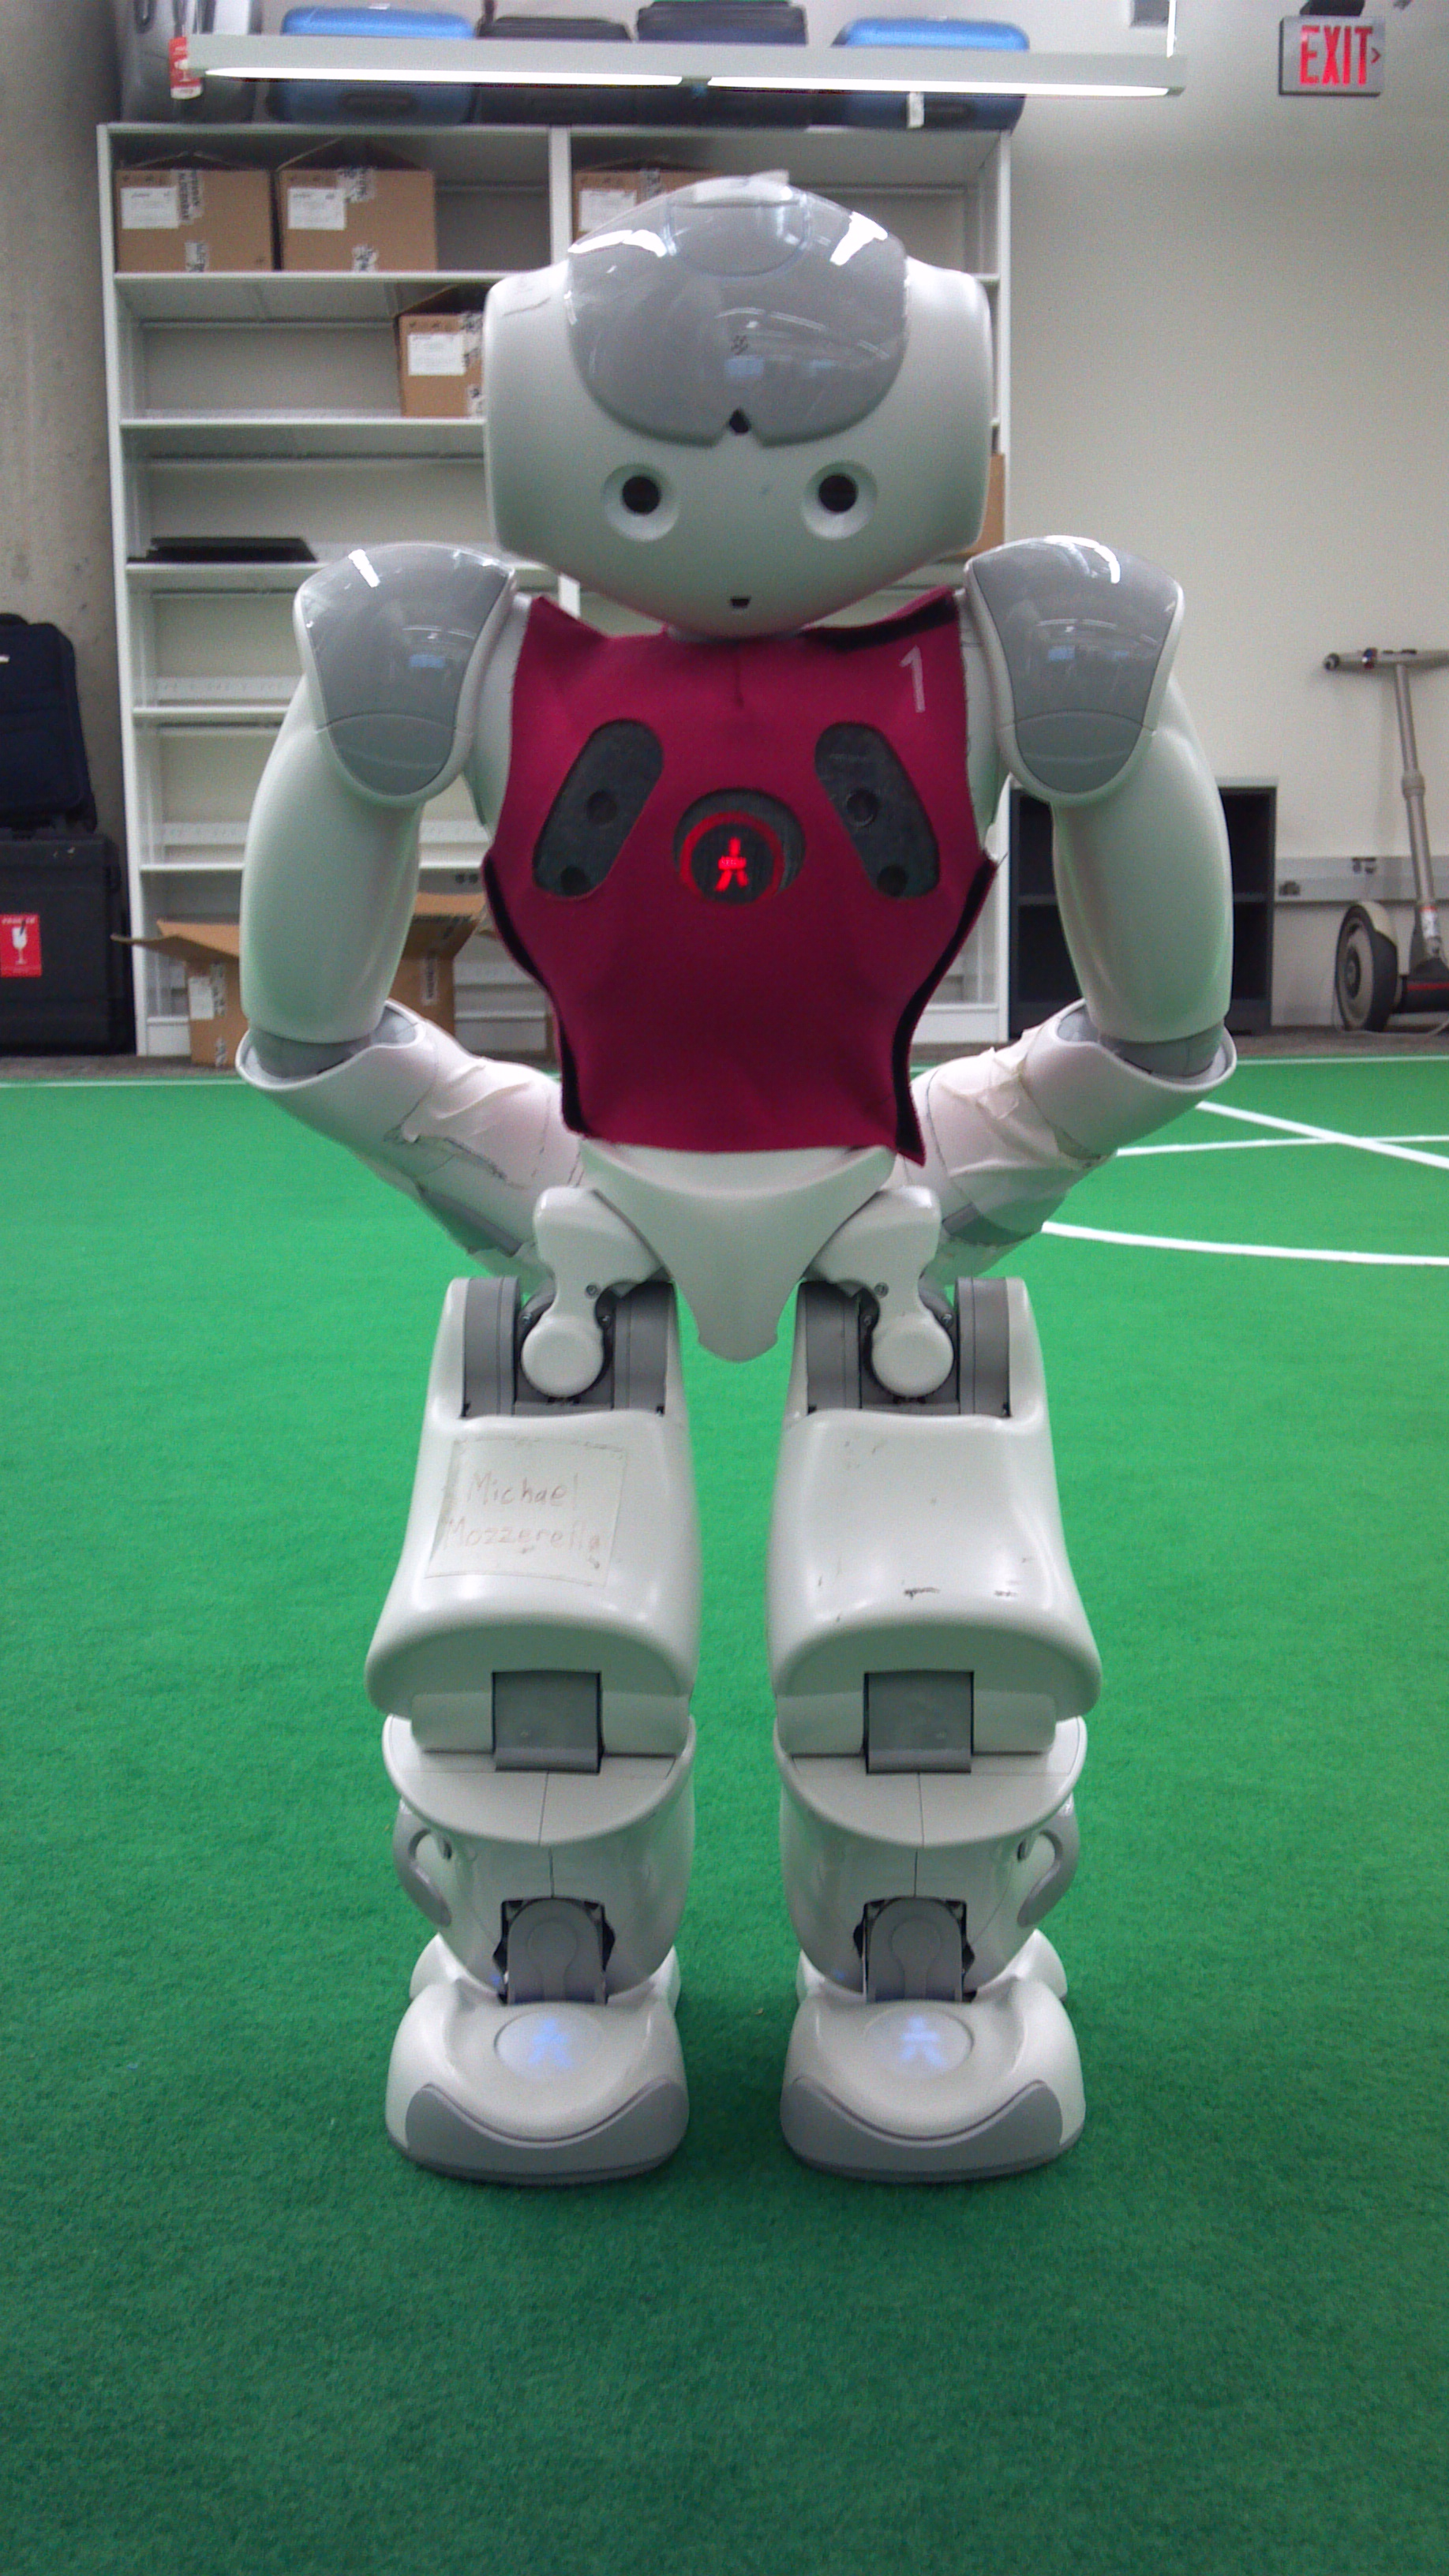
\includegraphics[height=0.28\columnwidth]{figs/front.jpg}&
      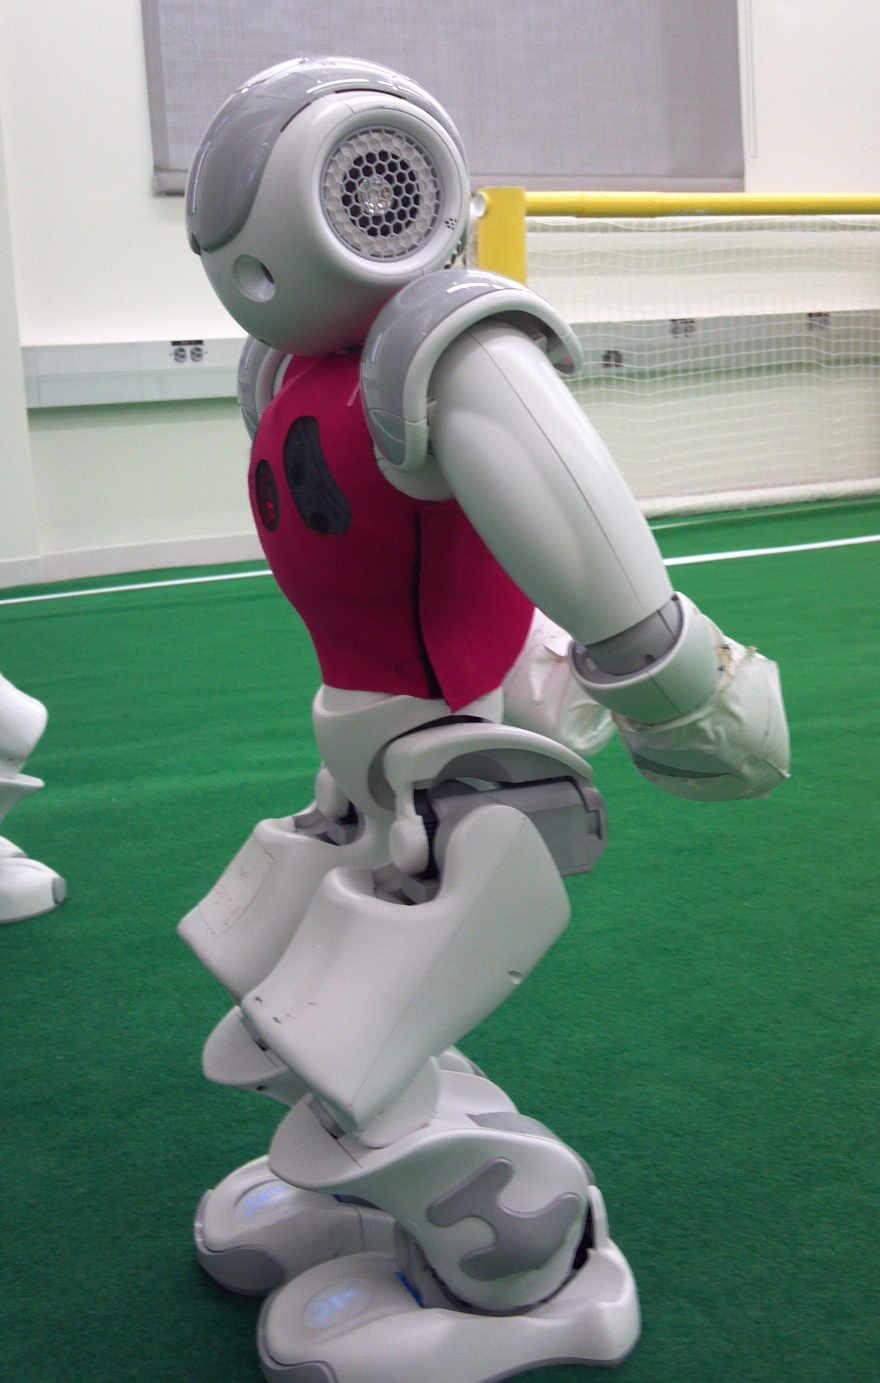
\includegraphics[height=0.28\columnwidth]{figs/side.jpg} &
      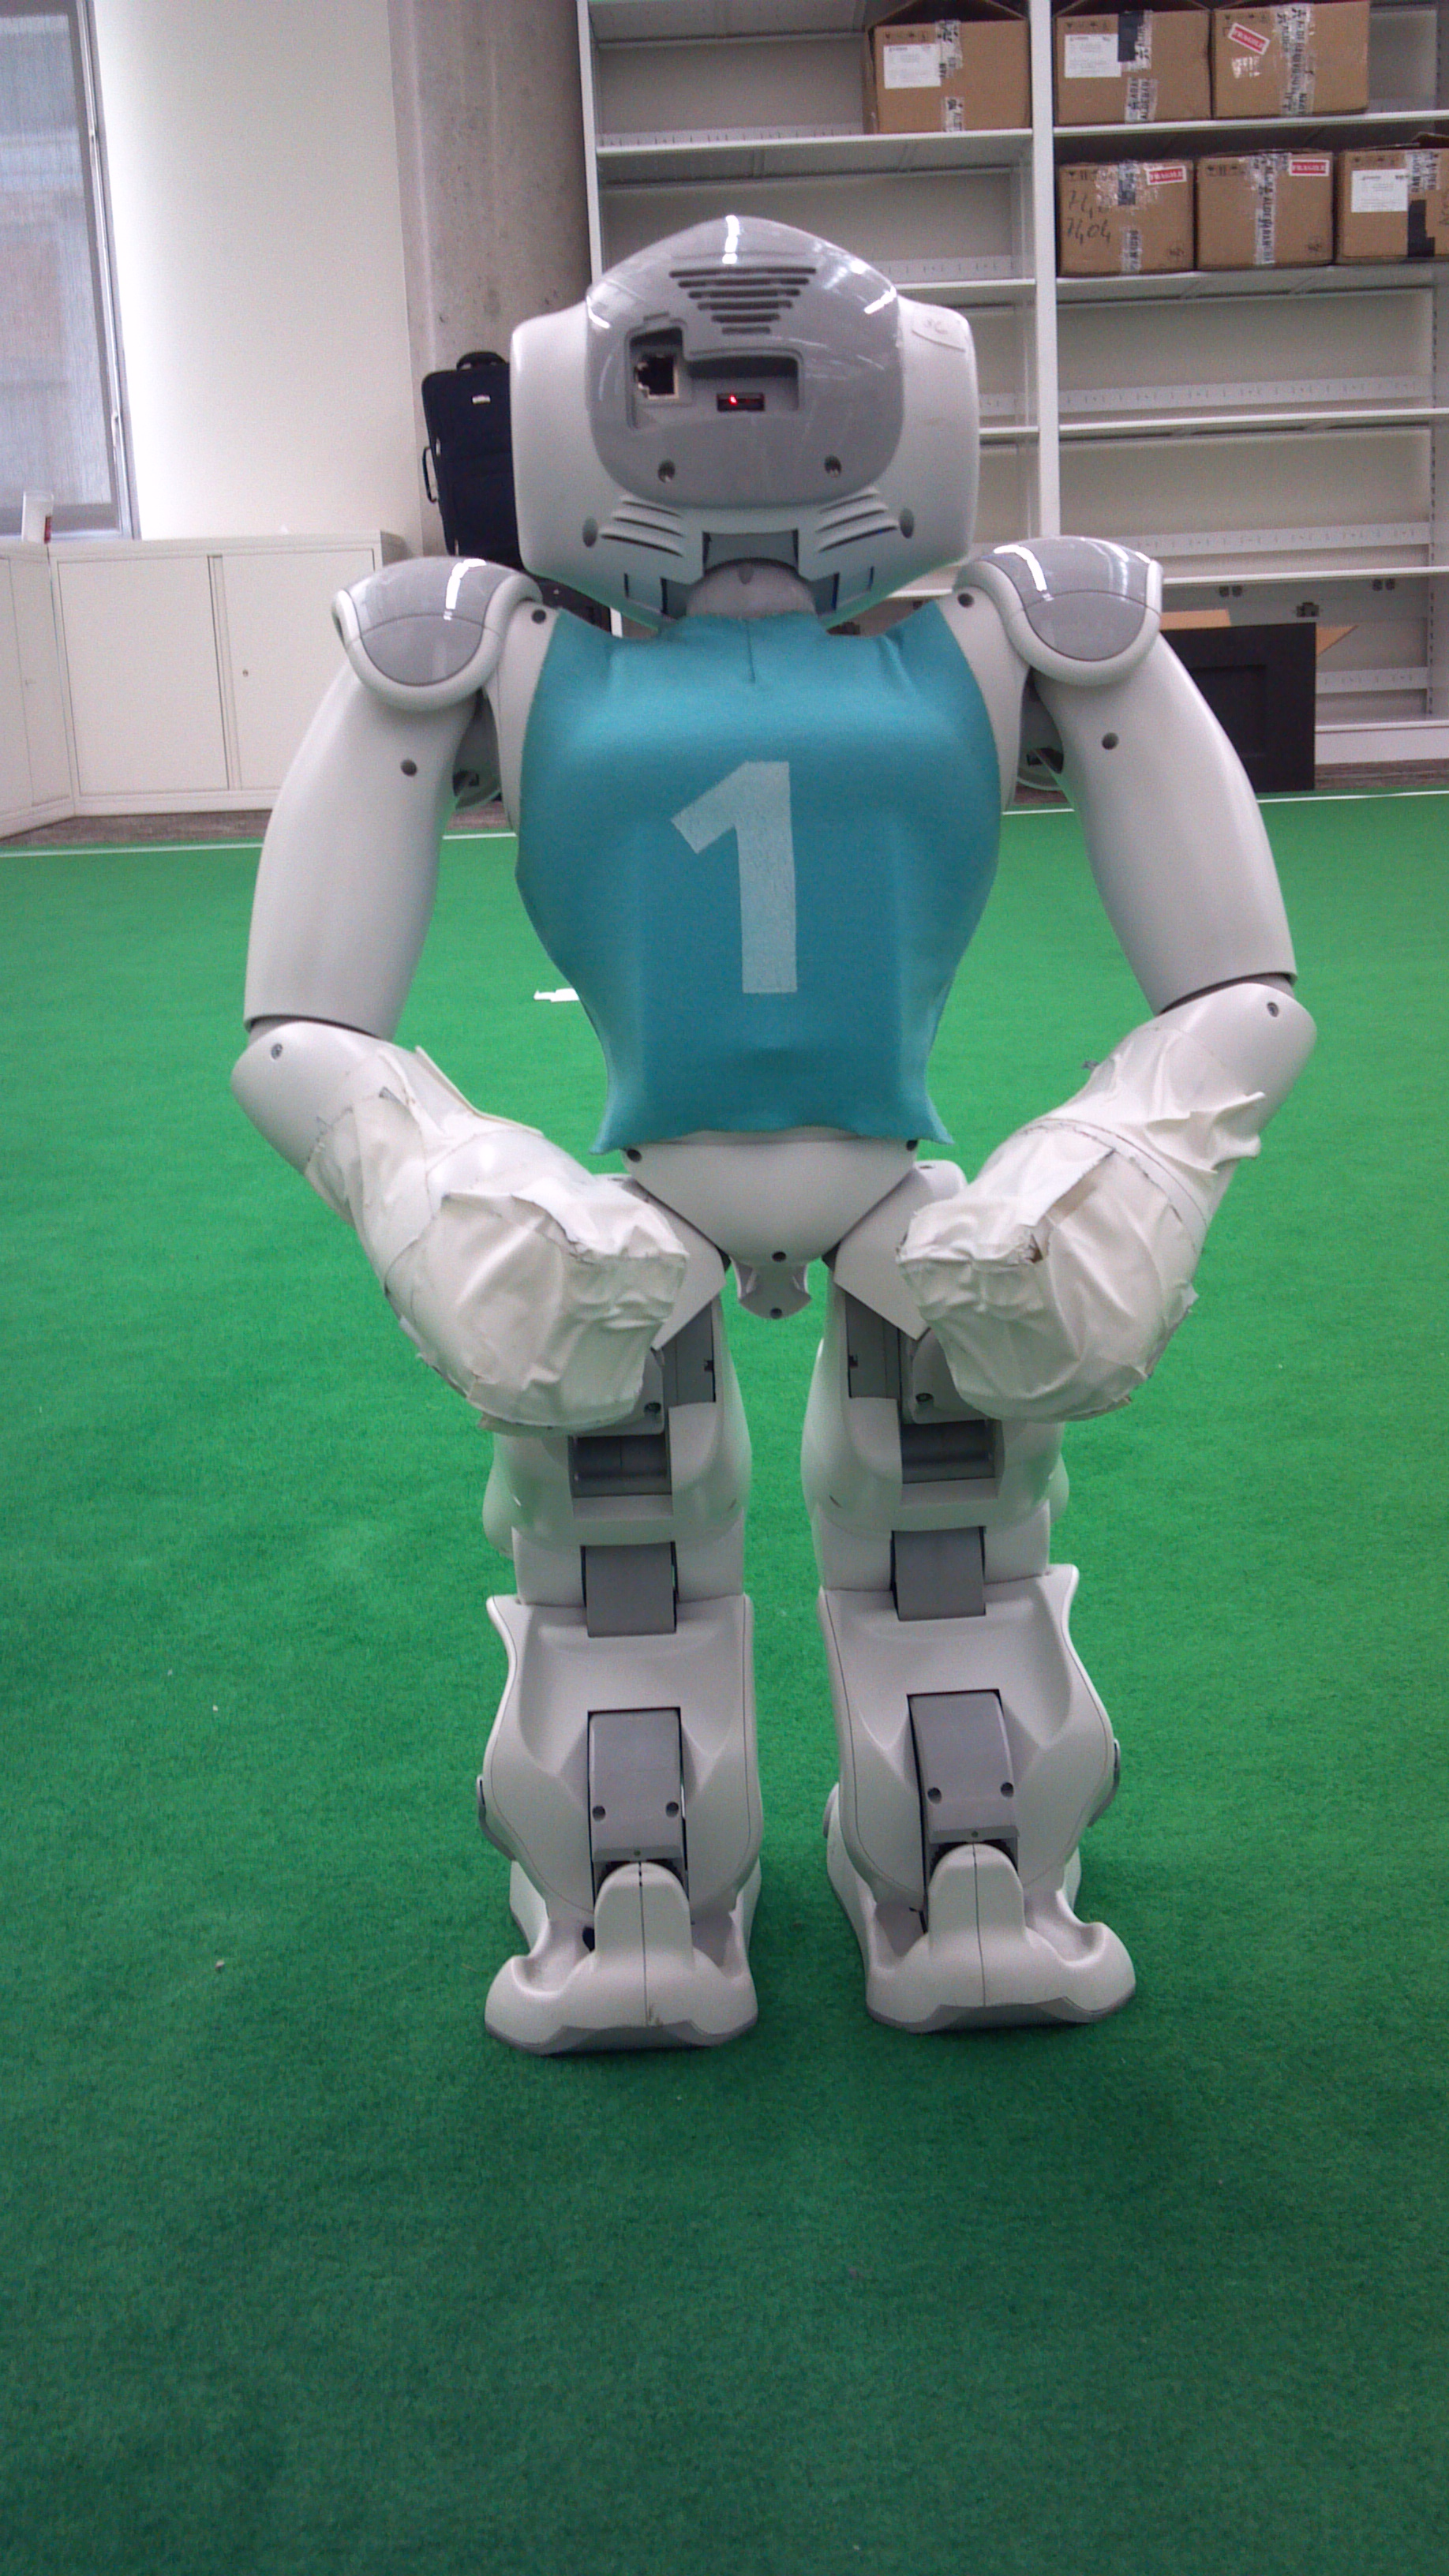
\includegraphics[height=0.28\columnwidth]{figs/back.jpg} 
  \end{tabular} }
  \caption{Team markers. a) Front view. b) Side view. c) Back view.} \label{fig:nao_markers}
\end{figure}

Teams may attach, print, or sew sponsor or team logos to the official jersey shirts.  One acceptable location is centered above the number on the back of the jersey, while the other acceptable location is on the front of the jersey, opposite to the team number, as depicted in Fig. \ref{fig:sponsor_jersey}.

Logos in one of two styles are allowed.  The first style would be a white background with a black or gray print.  The second style would be one in which a white, gray, or black logo is screen-printed on the jersey, such that the background of the logo is the jersey.  In either case, the dimensions of the logos are limited: the back logo has a maximum height of 3 cm and a maximum width of 8 cm, the front logo has a maximum height of 3 cm and a maximum width of 3 cm.

The coaching robot is allowed to wear a custom shirt that has a team-specific design. There are no restrictions regarding colors or patterns. The shirt is allowed to cover the body as well as the upper arms of the coaching robot.

\begin{figure}[b]
\centerline{\begin{tabular}{ll}
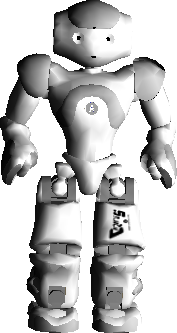
\includegraphics[height=0.35\columnwidth]{figs/naosim_with_logo.png}&
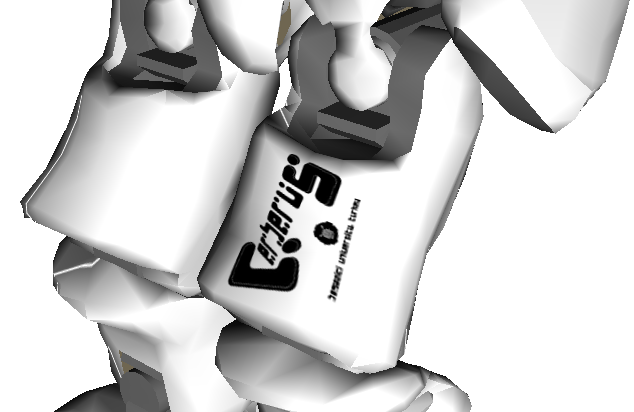
\includegraphics[height=0.35\columnwidth]{figs/naosim_legs_with_logo_closeup.png}
\end{tabular}}
\caption{Example Sponsor/Team Logo placement on legs.}
\label{fig:sponsor}
\end{figure}

\begin{figure}
\centerline{
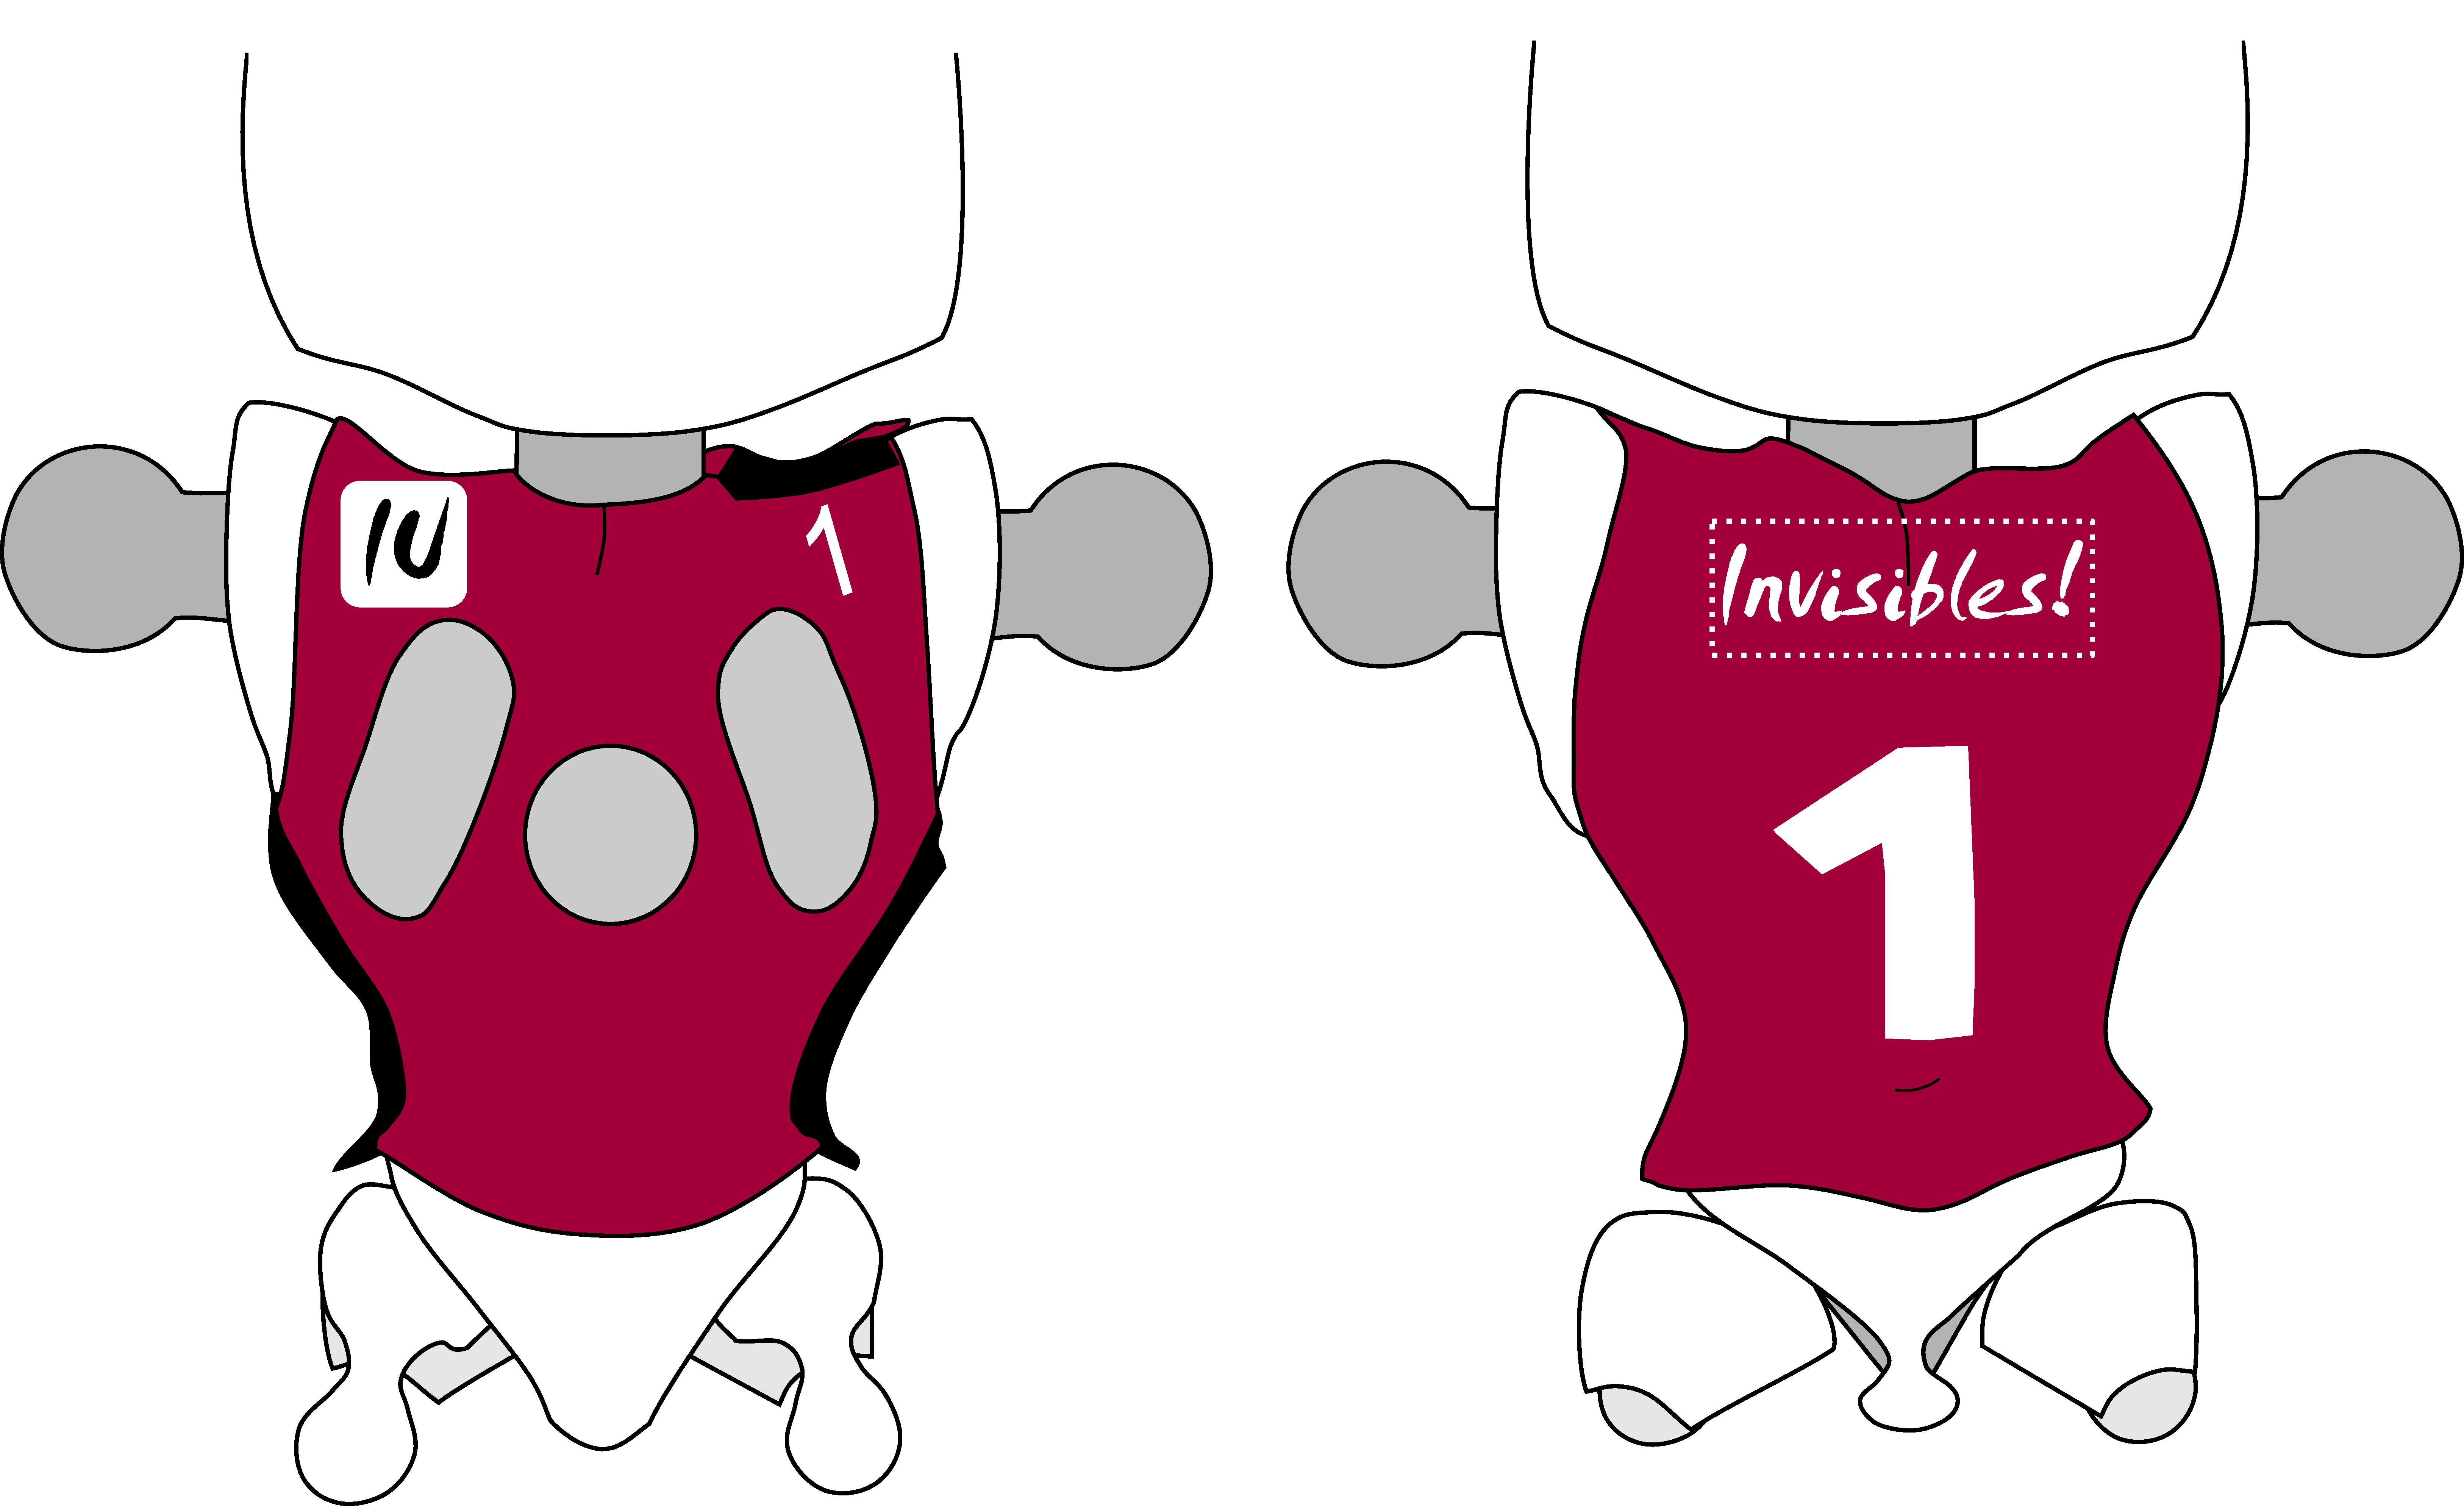
\includegraphics[width=0.7\textwidth]{figs/jersey-logo.pdf}}
\caption{Example Sponsor/Team Logo placement on jerseys.}
\label{fig:sponsor_jersey}
\end{figure}


\subsection{Communications}

The robots should play without human control. Communication is only allowed among robots on the field and between the robots and the GameController.

\subsubsection{Acoustic Communications}

There are no restrictions on communication between the robots using a microphone or a speaker.

\subsubsection{Wireless Communications}
\label{sec:wireless}
The only wireless hardware allowed to be used by the teams are the wireless network cards built into the NAOs, and the access points provided by the event organizers. All other wireless hardware must be deactivated. A team may be disqualified if one of the team members violates this rule. The MAC-addresses of all NAOs participating in the competition will be registered. Only these MAC-addresses can be reached through the access points provided by the event organizers. In addition, the access points will be secured by different SSIDs and WEP keys. 

Each team will get a range of IP addresses that can be used both for their robots and their computers. The IP addresses, channels, SSIDs, and WEP keys of the fields will be announced at the competition site.

Wireless robot-to-robot communication among the robot players is allowed, as long as it uses the access points provided by the event organizers (using the so-called ad-hoc mode is prohibited), messages are sent via UDP, the SPL standard message packet is used, and not more than five messages (excluding return packets to the GameController) per robot per second are sent. The SPL standard message packet is specified in \url{https://www.tzi.de/spl/pub/Website/Downloads/SPLStandardMessage.h}. Each team will be assigned a range of IP-addresses that can be used for direct robot-to-robot communication. Each team will also be allocated a limited range of UDP ports on which broadcast will be permitted.

The GameController will use UDP to connect to the robots. The source distribution of the GameController provides the header file \emph{RoboCupGameControlData.h} that defines all messages sent by the GameController to the robots. They correspond to the \emph{robot states} described in Section~\ref{sec:robot_states}.

The coaching robot is not allowed to communicate directly with the robot players, \ie it is neither allowed to send any messages to the players nor is it allowed to listen on ports that are used by players to send messages. Instead, it sends messages to the GameController's coaching interface by using the struct defined in \url{https://www.tzi.de/spl/pub/Website/Downloads/SPLCoachMessage.h}. These messages have a maximum size of 20 bytes and will be copied by the GameController to its standard messages. However, independent of the sending frequency of a coach, the GameController will accept a new message only every 10 seconds --- all other coach messages will be dropped. In addition, the update of the coach message will be delayed by the GameController by about 8--12 seconds (the exact offset is determined randomly for each message). This represents the intent that the coaching robot should make long-term strategic decisions instead of immediately controlling the robot players. It is intended to display the coach messages to the audience, \eg via the GameController display. Therefore, these messages have to be in a human-readable\footnote{In this context, the definition of ``human-readable'' is: There exist humans outside the RoboCup context who can easily understand the content of the message, \ie it is not required to use any specific language (such as English) and teams could use, for instance, their native language.} format and may not contain any numbers.  Failure to follow these specifications will result in the inability to use the coaching robot until it is able to follow these specifications.

The use of remote processing/sensing is prohibited.


\newpage


\section{Game Process}
\label{sec:game_process}

\subsection{Structure of the Game}
\label{sec:game_struct}

A game consists of three parts, \ie the first half, a half-time break, and the second half. Each half is 10 minutes counted from the initial kick-off. The half-time break is also ten minutes --- during this time both teams may change robots, change programs, or do anything else that can be done within the time allotted. 

The teams will change the goal defended during the half-time break.

\begin{figure}[t]
\centerline{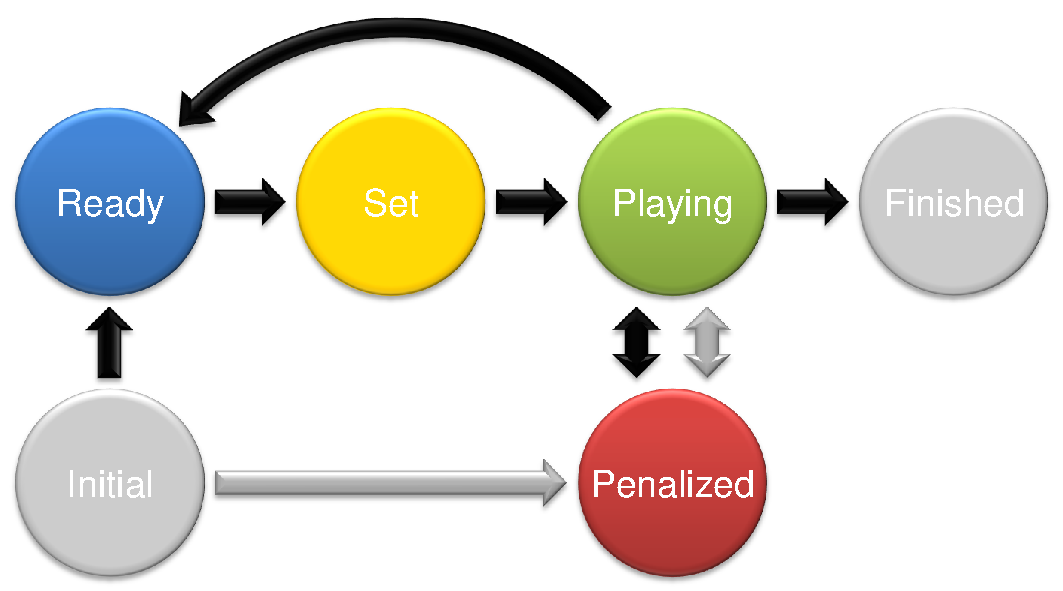
\includegraphics[width=0.9\columnwidth]{figs/states.pdf}}
\caption{Robot states. Button interface transitions are shown in gray. GameController transitions are shown in black. However, any transition possible can actually be sent by the GameController.}
\label{fig:robot_states}
\end{figure}

\subsection{Robot States}
\label{sec:robot_states}

Robots can be in six different states (\cf Figure~\ref{fig:robot_states}). If the wireless is available, these states will be set by the GameController. Teams must implement code to receive and correctly respond to wireless GameController packets, and also give indication of the game state, team color, and the kickoff state.
\emph{If a robot does not respond to either the game controller or the button press interface, then it is not included in the game, and the game starts without the offending robot.}

\begin{description}

\item[Initial.] After booting, the robots are in their \emph{initial} state. In this state, the button interface for manually setting the team color and whether the team has kick-off is active. The robots are not allowed to be moving in any fashion besides initially standing up. Pressing the left foot bump sensor will switch the team color. Shortly pressing the chest button will switch the robot to the \emph{penalized} state.

\item[Ready.] In this state, the robots walk to their legal kick-off positions (\cf Section~\ref{sec:kick-off}). They remain in this state, until the head referee decides that there is no significant progress anymore (after a maximum of \KickOffAutoTime). This state is not available if only the button interface is implemented.

Robots may be disentangled by the referees at the start of the Ready state. After that, 
the ``Player Pushing'' rules are applied, but the penalty is manual placement by the assistant referees (\cf Section~\ref{sec:kick-off}), not the penalty described in Section~\ref{sec:player_pushing}.
Consequently those pushings do not go into the permanent removal count.

\item[Set.] In this state, the robots stop and wait for kick-off (\cf Section~\ref{sec:kick-off}). If they are not at legal positions, they will be placed manually by the assistant referees to the positions shown in Figure~\ref{fig:ko}. They are allowed to move their heads before the game (re)starts but they are not allowed to move their legs or locomote in any fashion. This state is not available if only the button interface is implemented. Robots that do not listen to the GameController will be placed manually. Until the game is (re)started, they are in the \emph{penalized} state.

\item[Playing.] In the \emph{playing} state, the robots are playing soccer. Shortly pressing the chest button will switch the robot to the \emph{penalized} state.

\item[Penalized.] A robot is in this state when it has been penalized. It is not allowed to move in any fashion, \ie also the head has to stop turning. Shortly pressing the chest button will switch the robot back to the \emph{playing} state.

\item[Finished.] This state is reached when a half is finished. This state is not available if only the button interface is implemented.

\end{description}

The team color should be displayed during the whole game on the LED of the left foot (blue/red). Teams that support the GameController can visualize whether the robot's team has kick-off on the LED of the right foot (off/white) in the states \emph{initial}, \emph{ready} and \emph{set}. The current game state should be displayed on the LED in the torso. The colors corresponding to the game states are:

\begin{itemize}

\item Initial: Off

\item Ready: Blue

\item Set: Yellow

\item Playing: Green

\item Penalized: Red

\item Finished: Off

\end{itemize}

\subsection{Goal}

A goal is achieved when the entire ball (not only the center of the ball) goes over the goal-side edge of the goal line, \ie the ball is completely inside the goal area\footnote{The goal line is part of the field.}. The restart after the goal shall adopt the same rules as the kick-off.

Note that a goal can never be awarded where the last contact of the ball with a robot was by the arm or hand (see Section~\ref{sec:hand_ball}) of an attacking robot. Should the ball enter the goal area where the last contact is with the arm or hand of an attacking robot, the goal shall not count and a goal kick is awarded, that is, it shall count as if the ball is out by the attacking team (see Section \ref{sec:throw_in}).

\subsection{Goal Keeper Save}
\label{sec:goalie_save}
While within its penalty area, a goal keeper may touch the ball with its arms and/or hands.  If a goal keeper is able to lift the ball off of the ground using its arms and/or hands, and hold it there for at least 1 second, the ball will be moved to the intersection of a throw-in line and the halfway line.

The robot is not required to lift the ball to a particular height in order for the ball to be considered to be `lifted off of the ground', but lack of contact between the ball and ground must be clearly recognizable by the head referee.

\subsection{Applying Penalties}

See Section~\ref{sec:penalty_procedure}.


\subsection{Initial Kick-off}
\label{sec:initial-kick-off}

The first kick-off at the start of each half is the initial kick-off.
Before the initial kick-off, i.e. before the start of each half, all robots must be in the initial state and must be placed on the sidelines in their own half of the field.
It is up to the team as to which sideline(s) and where exactly on the sidelines the robots are placed.
Once the robots receive the \emph{ready} signal from the GameController, they are to proceed as described in Section~\ref{sec:kick-off}.


\subsection{Kick-off}
\label{sec:kick-off}
For kick-off, the robots listening to the wireless GameController run through three states: \emph{ready}, \emph{set}, and \emph{playing}. Robots not listening to the GameController are simply penalized and manually placed for kick-off\footnote{Note that robots being manually placed because they are not listening to the GameController must still be placed in the restricted set of legal positions for manually placed robots. It is to a team's advantage to have their robots listen to the GameController.}.

In the ready state, the robots should walk to their legal kick-off positions. These positions are always located inside their own side of the field. No player is allow to touch the halfway line.
The field players of the attacking team can walk to any position within their own half (including inside the center circle), except for inside the penalty area.
The field players of the defending team can walk to any position within their own half, except for inside the center circle and the penalty area.
The feet of both goal keepers must be \emph{inside} the penalty area.

If robots collide during the Ready state, the ``Player Pushing'' rules are applied, but the penalty is manual placement by the assistant referees, not the penalty described in Section~\ref{sec:player_pushing}.
Consequently those pushings do not go into the permanent removal count.

The robots have a maximum of \KickOffAutoTime to reach their positions. If all the robots have reached legal positions and have stopped, or if \KickOffAutoTime have passed, the robots will be switched into the \emph{set} state, in which they must stop walking. Each robot that is not at a legal position at this point in time will be placed manually by the assistant referees to the positions as shown in Figure~\ref{fig:ko}. Robots that are legally positioned will not be moved by the assistant referees unless a manual position is requested by the team leader.
\emph{In the case where the team leader requests manual placement, all robots on that team are manually positioned.}


\begin{figure}[t]
\centerline{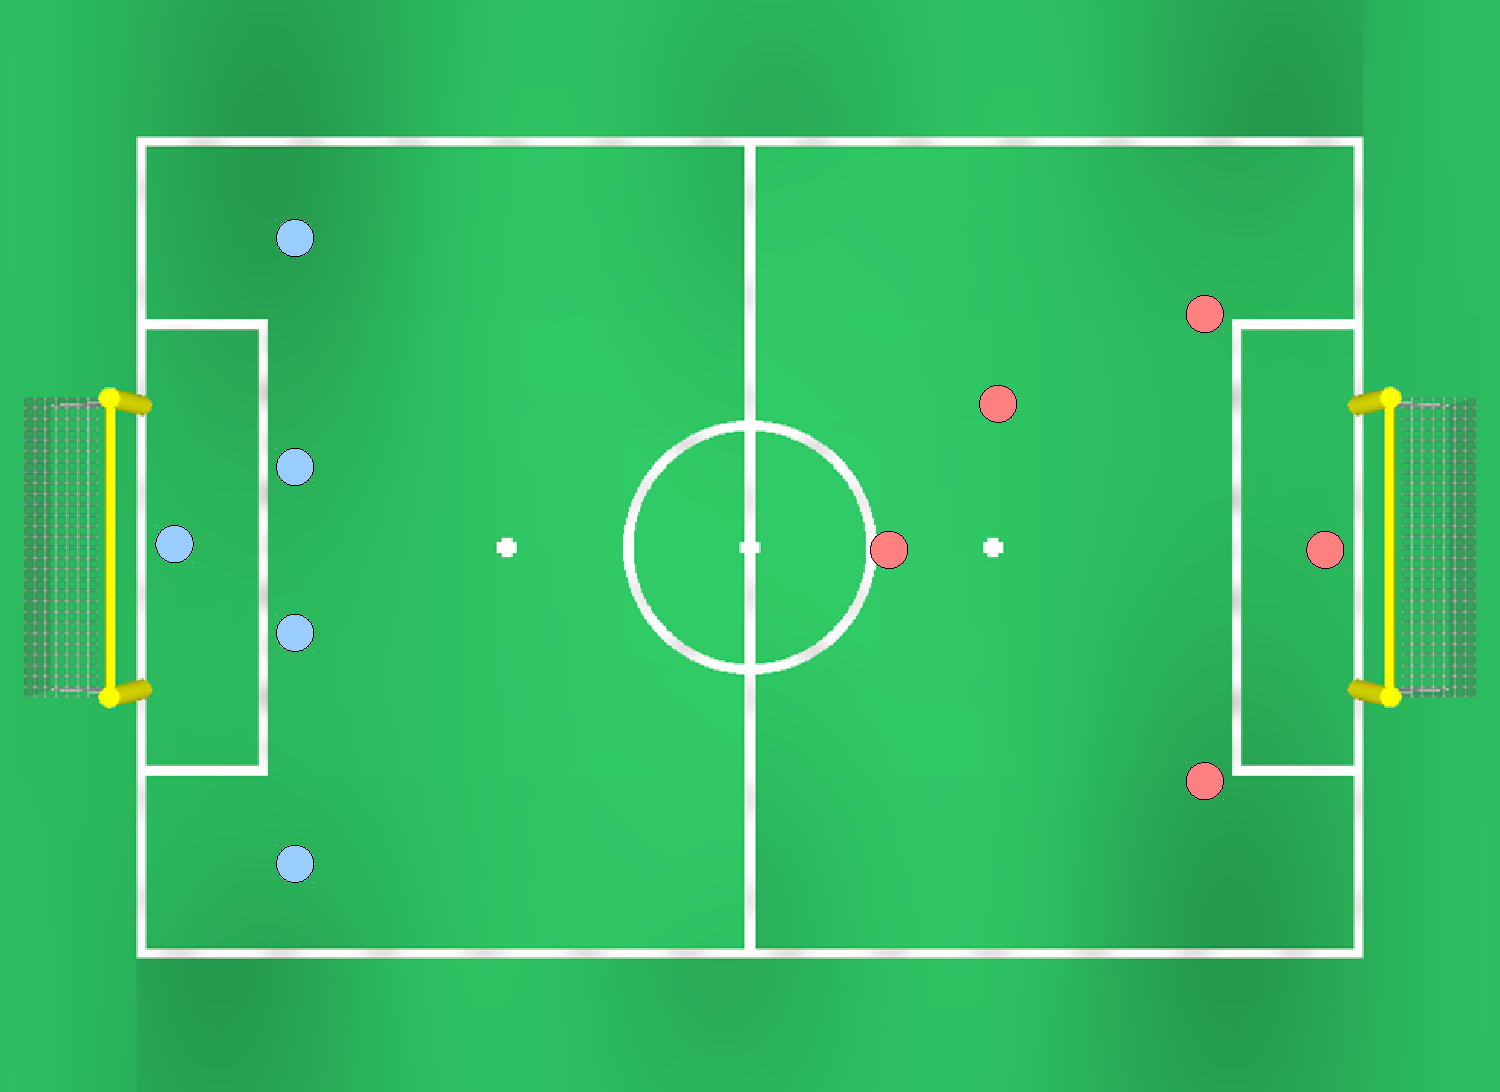
\includegraphics[width=\columnwidth]{figs/manual_placement_2013.pdf}}
\caption{Manual setup for kick-off.  The attacking team is on the right.}
\label{fig:ko}
\end{figure}

There are extra restrictions on the legal positions of manually positioned robots. The kicking-off robot is placed on the center circle, right in front of the penalty mark. Its feet touch the line, but they are not inside the center circle. 
One of the other field players of the attacking team is placed in front of one of the goal posts on the height of the penalty mark (i.e. the virtual intersection point of the goal post and the penalty mark) and the other two are placed on the corners of the penalty box without having their feet touching the corners. 
Two field players of the defending team are placed halfway between the corners of their own penalty box and the sidelines. The other two field players of the defending team are placed immediately in front of their own penalty box, halfway between the center of the penalty box and the goal post.  The goal keepers for each team are placed at the center of the penalty box, with their feet immediately in front of the end-line.

To assist the assistant referees in placing the robots manually when needed or requested, small Ks and Ds will be marked on the field using a black felt-tip pen in the spots where manually placed robots should go if they are kicking off (Ks) or defending (Ds).  These marks should be small, such that they are visible to humans but invisible to robots.

As autonomously placed robots are allowed to be much closer to the ball, successful autonomous placement results in a significant advantage over manual placement.

Just before the \emph{set} state is called, the ball is placed on the center point of the center circle by one of the referees. If it is moved by one of the robots before set is called it is replaced by one of the referees.

After the head referee has signaled the kick-off, the robot's state is switched to \emph{playing} (again either by the GameController or manually), in which they can actually play soccer.
The defensive team must stay outside of the center circle until the ball is in play.  The ball is in play once it is touched by the attacking team or once \emph{10 seconds} have elapsed in the playing state. If a defensive player enters the center circle before the ball is in play the ``Illegal Defender'' penalty is applied (\cf Section~\ref{sec:illegal_defender}).

Note that a goal can never be scored directly from a kick-off shot. See Section~\ref{sec:kick-off_shot} for details.

The current GameController requires robots to know both their team number and their robot number within the team. It is each team's responsibility to make sure this is correctly configured. It is recommended that the robot indicates its number within the team on bootup so that this can be easily checked at the start of the game.

\subsection{Throw-in}
\label{sec:throw_in}

A ball is considered to have left the field when there is no part of the ball over the outside of the boundary line (\ie the line itself is in). If the ball leaves the field it will be replaced on the field by an assistant referee. There is \emph{no} stoppage in play.

If the ball goes over a sideline then the assistant referee will replace the ball back on the field on the throw-in line on the same side of the field as the ball went out of play.

The ball will be replaced on the throw-in line at the farthest back of these two locations: a) one meter back from the point it went out or b) one meter back from the location of the kicking robot. We define `back' as being towards the goal of the team that last touched the ball. Note that if the one meter placement would cause the ball to be placed off the end of the throw-in line, then it should be placed at the end of the throw in line, and not beyond.

If the ball goes over an end-line then the assistant referee will replace the ball back on the field according to the following rules:

\begin{itemize}

\item If the ball was last touched by the defensive team then the ball is replaced on the closest endpoint of the throw-in line.

\item If the ball was touched by the offensive team, the ball is replaced on
the throw-in line at the farthest back of these two locations: a) one
meter back from the location of the kicking robot, or b) at the halfway
line.

\end{itemize}

Balls are deemed to be out based on the team that last touched the ball, irrespective of who actually kicked the ball.  In these examples, ``yellow half of the field'' refers to the half the yellow team is defending.

\paragraph{Example 1.} The red goal keeper kicks the ball out the end of the field to the right of the goal. The ball is placed on the endpoint of the throw-in line to the right of the goal.

\paragraph{Example 2.} A blue robot on the yellow half of the field kicks the ball out the end of the field to the right of the goal the red team is defending. The ball is placed on the intersection of the right throw-in line and the halfway line.

\paragraph{Example 3.} A blue robot on the blue half of the field kicks the ball out the end of the field to the right of the goal the red team is defending. The ball is placed on one meter behind the robot on the right throw-in line.

\paragraph{Example 4.} A blue robot at midfield kicks the ball over the left sideline 2 meters into the yellow half of the field. The ball is replaced on the left throw-in line 1 meter into the blue half of the field (one meter behind the robot).

\paragraph{Example 5.} A blue robot at midfield kicks the ball over the left sideline 2 meters into the blue half of the field (towards its own goal). The ball is replaced on the left throw-in line 3 meters into the blue half of the field.

\paragraph{Example 6.} A blue robot kicks the ball but the ball touches a red robot at midfield before leaving the field near the centre line. The ball is regarded as out by red and therefore is replaced on the throw-in line 1 meter closer to the goal the red team is defending.


\subsection{Game Stuck}
\label{sec:game_stuck}

In the event of no substantial change in the game state for 15 seconds, this is considered a game stuck. 
This includes if a robot is at the ball circling it for 15 seconds without kicking the ball.
The main referee has two options how to solve the game stuck and to reestablish the chance of progress in the game. The intention of the game stuck rule is to achieve progress with as little intervention as possible, \ie the \emph{Local Game Stuck} rule will be preferred, but only if there is a chance that its application will result in progress in the game.

\subsubsection{Local Game Stuck}
\label{sec:game_stuck:local}

The nearest robot to the ball will get the standard removal penalty according to Section~\ref{sec:removal_penalty}.

\subsubsection{Global Game Stuck}
\label{sec:game_stuck:global}

The referee stops the game and restarts the game from the kick-off formation. The kick-off will be awarded to the team defending the side of the field the ball is on when the game stuck is called. A global game stuck can only be called if at least one robot has touched the ball since the previous kick-off.

\subsection{Request for Pick-up}
\label{sec:request_for_pickup}

Either team may request that one of their players be picked up only for hardware dysfunction and software crashes at any point in the game (called ``Request for Pick-up''). 
Basically every change (hardware or software) is allowed during a request for pick-up. In particular,
it is permitted to change batteries, fix mechanical problems, reboot the robots, and change configuration files.
It is discouraged to change the robot's control program, \textbf{but not forbidden}.
It is also allowed to replace a broken robot by a substitute robot.

Any strategic ``Request for Pick-up'' is not allowed, i.e. gaining an advantage by removing the robot from the game.
In general, a ``Request for Pick-up'' for a robot which is currently in the game is only allowed for obvious hardware failures.
In this case, the head referee will indicate when the robot is no longer affecting play and can be removed from the field by an assistant referee.
A ``Request for Pick-up'' for a robot which is currently out of the game, e.g. penalized, can be granted immediately.

To prevent mistakes and confusion during games, only team leaders should make a ``Request for Pick-up'', and only one designated person per team shall accept the robot from the referee, and hand it back after fixing the problem.
The returning robot will be replaced after a minimum of 45 seconds after it was taken off the field following the normal replacement procedure used after the standard removal penalty (see Section~\ref{sec:removal_penalty}).

If a robot has been rebooted and the wireless is not working, it is the responsibility of the team members (not the assistant referees) to configure its team color correctly. The robot should be returned to the assistant referees in the \emph{penalized} state so that the assistant referees cannot accidentally change the robot's team color.

\subsection{Request for Timeout}
\label{sec:request_for_timeout}

At any stoppage of play (after a goal, stuck game, before half, etc.) either team may call a timeout. Each team can call a \textbf{maximum of 1 timeout per game} with a total time totaling no more than \textbf{5 minutes}. During this time, both teams may change robots, change programs, or anything else that can be done within the time allotted. 
The timeout ends when the team that called the timeout says they are finished, at which time they must be ready to play. The other team must be ready to play at the time the timeout runs out, or \textbf{2 minutes} after a prematurely called end of the timeout, whichever is earlier. If the other team is not ready to play in time, it has to call a timeout of its own.
  
The clock stops during timeouts, even during the preliminaries.

After the completion of the timeout, the game resumes with a kick off for the team which did not call the timeout.

If a team is not ready to play at the assigned time for a game, the referee will call the timeout for that team. After the expiration of such a timeout, if the team is still not ready to play then the referee shall start the game with only one team on the field.  The team that wasn't ready can return its robots to the field as per the rules for ``Request for Pick-up''. If both teams are not ready, the referee will call timeouts for both teams. This ``double timeout'' expires after 10 minutes.

\subsection{Referee Timeout}
\label{sec:referee_timeout}
The head official may call a timeout at any stoppage of play if he or she deems it necessary.  A referee timeout should only be called in dire circumstances --- one example might be when the power to the wireless router is down.  However, when and whether to call a referee timeout is left up to the head referee.

Referees may call multiple timeouts during a game if needed.  Teams may do anything during these timeouts, but they must be ready to play \textbf{2 minutes} after the referee ends a timeout.  The referee should end the timeout once he or she believes the circumstance for which the timeout was called has been resolved.  In cases where the circumstance for which the timeout was called is not resolved within 10 minutes, the chair of the technical committee should be consulted regarding when/if play should continue.

The team who would have kicked off if the timeout had not been called shall kickoff when the game resumes.

\subsection{Rules for Forfeiting}
\label{sec:forfeit}

If a team chooses to forfeit a match then the opposing team will play the match against an empty field.  However, any own goals will not be scored.  Hence, after an opponent forfeits, the team playing against an empty field cannot do worse than they were doing at the time the opponent decided to forfeit.  Teams may choose to forfeit a game at any stage.  However, once a forfeit is announced, they may not reverse this decision.


\subsection{Penalty Kick Shoot-out}
\label{sec:penalty_shoot-out}

A penalty kick shoot-out is used to determine the outcome of a tied game when an outcome is required (for example, during the intermediate round, quarter finals, semi finals, third place or final). 
There will be a five minute break between the end of the game and the start of the penalty kicks.
In the intermediate round, the penalty kick shoot-out will consist of three penalty shots per team; in the quarterfinals and later, it will consist of five penalty shots per team.
All penalty shots are taken against the same goal\footnote{Which goal to take for the shoot-out is decided in accordance with the teams, or otherwise by a coin toss.}. At the conclusion of these shots the team that has scored the most goals will be declared the winner. Note that a winner can be declared before the conclusion of the penalty shoot-out if a team can no longer win, for example, a team requires 3 goals to win but only has 2 attempts remaining. If the two teams still remain tied then a sudden death shoot-out will follow until a definite winner is found.

The procedure for each attempt is described in Section~\ref{sec:penalty_kick}. For the first five attempts, the standard time limit of 1 minute is applied. If after five penalty kicks by each team there is no result (that is, each team has scored the same number of goals), then the decision will be made by the following sudden death shoot-out procedure.

\subsubsection{Penalty Kick}
\label{sec:penalty_kick}

A penalty kick is carried out with one attacking robot and one opposing goal keeper. Other robots (including the coach) should be powered off and stay outside of the field. Teams are allowed to switch to specially designed software for a penalty kick. 

The ball is placed on the penalty spot, at the end of the field closest to the goal being defended. The attacking robot is positioned 1 meter behind the penalty spot, facing the ball.  This spot is denoted with a small dot made with a felt-tip pen. The goal keeper is placed with its feet on the goal line and in the center of the goal.

Neither robot shall move their legs before the penalty kick starts. Movements of the robot's head and arms are allowed as long as the robot does not locomote. Technically, the robots are in the \emph{set} state when waiting for the penalty kick to start. If robots are not listening to the GameController, they are in the \emph{penalized} state instead. The robots are started by switching to the \emph{playing} state.

The attacking robot is only allowed to contact the ball once.  The time limit for the kicker is 1 minute after the penalty kick starts. The ball must be in the goal within this time limit in order to count as a goal.

Hence, a penalty shot is over when the ball has come to a full stop after the first contact by the attacking robot, either in favor of the attacker if a goal has been scored, or in favor of the defending team if the goal keeper successfully blocked or if the ball just did not reach the goal line.

The goal keeper is not allowed to touch a ball that is completely outside the penalty area, where the line is part of the penalty area. If the goal keeper touches the ball when the ball is completely outside the penalty area, then a goal will be awarded to the attacking team.

All the rules such as ``Ball Holding'', ``Pushing'' and others are also applied during the penalty kick.  A goal keeper will not be penalized for inactivity during a penalty kick, provided its stiffness is on. Other penalties are applied as usual.

The attacking robot will be indicated by the GameController using the kick-off flag, \ie the kick-off team is the attacking one.

\subsubsection{Sudden Death Shoot-Out}

The time limit for sudden death penalty shots is two minutes.

These attempts will be timed (that is, for a goal scored, how long did it take to score the goal) and measured (that is, if a goal is not scored, what is the shortest distance between the ball and the goal line segment between the goal posts, achieved at any time during the penalty shot) by the referee. After these attempts, the game decision will be made as follows:

\begin{enumerate}

\item If only one team scores a goal, that team wins.

\item If both teams score a goal, then if one team is timed to have scored at least 2 seconds faster than the other team, the faster team wins. Otherwise, the sudden death shoot-out is repeated.

\item If neither team scores a goal, then if one team is measured to have moved the ball more than 50~mm closer to the goal than the other team, the closer team wins. Otherwise, the sudden death shoot-out is repeated.

\item If neither team has touched the ball during the shoot-out, the referee will toss a coin to decide the game.

\end{enumerate}


\newpage


\section{Forbidden Actions and Penalties}
\label{sec:forbidden_act}

The following actions are forbidden. In general, when a penalty applies, the robot shall be replaced, not the ball. For penalties that are timed, the penalty time is considered to be over whenever the game time stops (for goals, half-time, and game stuck).

\subsection{Locomotion Type}
\label{sec:locomotion_type}

Robots should clearly demonstrate bipedal walking similar to human walking. Other types of locomotion involving other parts than feet (crawling etc.) are strictly forbidden. It is duty of the head referee to decide whether a robot's locomotion is appropriate. Robots using inappropriate locomotion types will be removed via `Request for Pick-up' until they are able to show appropriate locomotion.

\subsection{Penalty procedure}
\label{sec:penalty_procedure}

When a robot commits a foul, the head referee shall call out the infraction committed, the jersey color of the robot, and the jersey number of the robot. The penalty for the infraction will be applied immediately by an assistant referee. The assistant referees should perform the actual movement of the robots for the penalty so that the head referee can continue focusing on the game. The operator of the GameController will send the appropriate signal to the robots indicating the infraction committed.

\subsection{Standard Removal Penalty}
\label{sec:removal_penalty}

Unless otherwise stated, all infractions in this league result in the removal of the infringing robot from the field of play for 45 seconds, after which it will be returned to the field of play. This process is called the standard removal penalty, and a detailed description of the process follows.

When the head referee indicates a foul has been committed that results in the standard removal penalty, the assistant referee closest to the robot will remove the robot immediately from the field of play. The robot should be removed in such a way as to minimize the movement of the other robots and the ball. If the ball is inadvertently moved when removing the robot, the ball should be replaced to the position it was in when the robot was removed.

The operator of the GameController will send the appropriate signal to the robot indicating the infraction committed. If the wireless is not working and the penalty is timed, the assistant referee handling the robot will reset the robot into the \emph{penalized} state for the duration of the penalty. After a penalty is signaled to the robot, it is not allowed to move in any fashion, such as being in the \emph{initial} state. The removed robot will be placed outside of the field facing away from the field of play.

The GameController will keep track of the time of the penalty. The operator of the GameController will signal the assistant referees when the penalty is 10 seconds from being over, so that one of them can place the robot in the half of the field which this robot's team is defending on the sideline that is farther from the ball. The robot should be placed close to the position where the penalty point projects on the sideline. This is illustrated in Figure~\ref{fig:penalty_re-entry_points}. 

If there is another robot already in this position, the robot should be replaced at a nearby location along the sideline. When finding a nearby location, locations away from the ball should be preferred, but they \textbf{must} still be in the robot's own half, so that the symmetry of the field can be resolved by the robot's localization system.

With approximatly 5 seconds left before the penalty ends, the robot should be turned to face towards the opposite sideline.

\begin{figure}[t]
\centerline{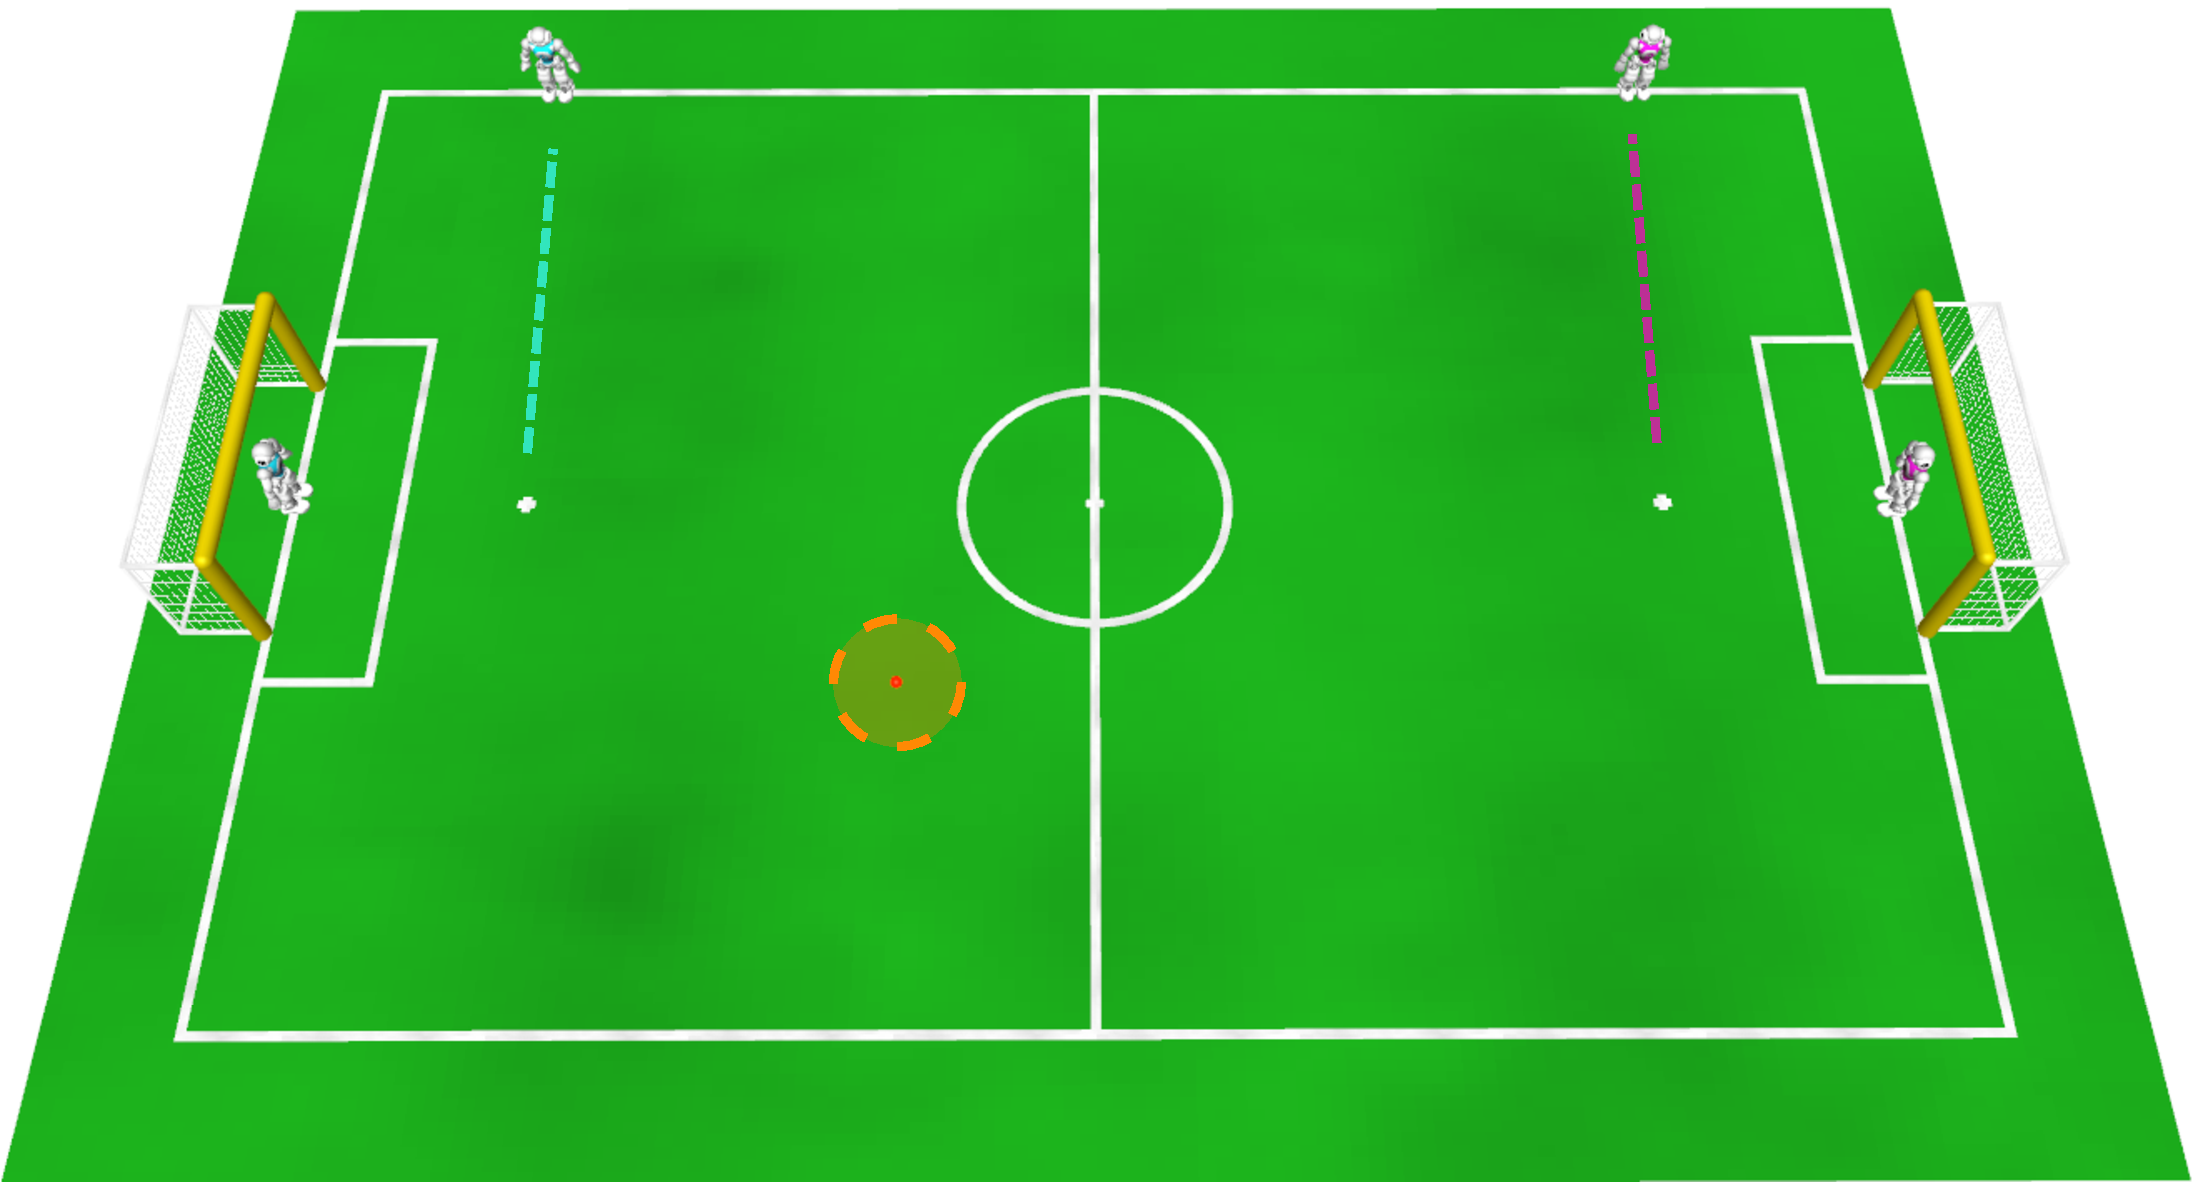
\includegraphics[width=\columnwidth]{figs/penalty_re-entry_points.pdf}}
\caption{For robots coming back from a standard removal penalty, re-entry points lie in their own half, on the sideline on the side away from the ball.}
\label{fig:penalty_re-entry_points}
\end{figure}

When the robot is on the field again, the operator of the GameController will send the \emph{playing} signal to it. If the wireless is not working, the assistant referee who placed the robot back on the field has to bring it into the \emph{playing} state again.

\subsection{Manual Interaction by Team Members}

Manual interaction with the robots, either directly or via some communications mechanism, is not permitted. Team members can only touch one of their robots when an assistant referee hands it over to them after a ``Request for Pick-up''.

\subsection{Kick-off Shot}
\label{sec:kick-off_shot}

A ``kick-off shot'' can never score a goal. A ``kick-off shot'' is a shot taken by the team kicking off after a kick-off before the entire ball has left the center circle, including the boundary line. 
If a kick-off shot enters the goal (either directly or via contact with an opposing robot), no goal will be scored and a kick-off will be awarded to the defending team (as per Section~\ref{sec:kick-off}).
The main referee's decision in this case is final and can not be changed afterwards by video proof.

\subsection{Ball Holding}
\label{sec:ball_holding}

The goal keeper is allowed to hold the ball for up to 5 seconds as long as it has one foot inside in its own penalty area.  If the goal keeper is attempting to grasp and lift the ball, it may hold the ball for up to 5 additional seconds. In all other cases (except those noted in Section \ref{sec:situations_no_ball_holding}), robots are allowed to hold the ball for up to 3 seconds. Holding the ball for longer than this is ``Ball Holding'' and is not allowed.

A robot which does not leave enough open space around the ball will be penalized as ``Ball Holding'' if that situation continues more than 3 seconds. The occupation of the ball is judged using the convex hull of the projection of the robot's body onto the ground. ``Enough open space'' means that at least the half of the ball is not covered by the convex hull. It is not important whether the robot actually touches the ball.

\begin{figure}[t]
\centerline{\begin{tabular}{ll}
a) & b) \\
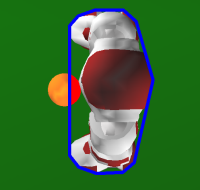
\includegraphics[scale=0.7]{figs/holding1} &
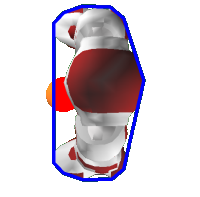
\includegraphics[scale=0.7]{figs/holding4}
\end{tabular}}

\caption{Examples for ``Ball Holding''. The orange circle is the ball, the blue polygon visualizes the convex hull of the robot's projection onto the ground and the red area shows the occupied portion of the ball. Situations a) is legal, whereas b) violates the rule.}
\label{fig:holding}
\end{figure}

Intentional continual holding is prohibited even if each individual holding time does not continue for up to the time limit. In general, robots should release the ball for approximately as long as they were holding it to reset the clock. Without a sufficient release, the continual holding is regarded as a continuous hold from the very beginning and the holding rule is strictly applied. The violation of this rule will result in the standard removal penalty (see Section~\ref{sec:removal_penalty} for details). The ball should be removed from the possession of the robot and placed where the foul occurred. If the robot that held the ball has moved the ball before the robot can be removed, the ball shall be replaced where the foul occurred.

\paragraph{Example.} A robot holds the ball and before the referees
can remove the robot, it shoots the ball into the goal. The goal
will not be counted and the ball will be replaced where the robot
held the ball.

\subsubsection{Exceptions to the Ball Holding Rules}
\label{sec:situations_no_ball_holding}

The following define situations where ball holding does not apply:

\begin{enumerate}
	\item Ball holding may not occur when the ball becomes stuck between a robot's legs.  An assistant referee should remove the ball in these situations and place the ball approximately where it was before it became stuck.
	\item Ball holding may not occur when a robot falls on a ball.  The robot will either get-up and hence free the ball, or the robot should be removed under the Fallen Robot rule.
\end{enumerate}


\subsection{Fallen or Inactive Robots}
\label{sec:fallenrobots}

If a robot falls during the game, it should start executing a getup action within 5 seconds. If it does not commence a get up action within 5 seconds, it will be removed as per the standard removal penalty. A robot which is unable to autonomously stand up within 20 seconds after a fall will be removed and subject to the standard penalty. The goal keeper, inside its own penalty area, is the only robot permitted to `dive' (that is deliberately fall in a way that might cause its torso, arms or hands) to intercept the ball. In all other cases, the robot should be programmed to attempt to remain upright -- that is, supported by its feet.

A robot that has ceased activity for 10 seconds or has turned off will be removed by the referees and is subject to the standard removal penalty. A robot is active if it performs at least one of the following:

\begin{enumerate}

\item The robot walks in any direction, or turns.

\item The robot searches for the ball, or is looking at the ball.

\end{enumerate}

\paragraph{Note:} The intention of this rule is not to penalize robots simply for being stationary -- provided they are not `asleep' and have not `crashed'.

\subsection{Player Stance}
\label{sec:player_stance}

Robots are not allowed to stay in a stance that is wider than the width of the robot's shoulders for more than 5 seconds. The robot is allowed to go into a wide stance as long as it comes back to a normal stance within 5 seconds. Staying in a wide stance for longer than 5 seconds will result in the standard penalty. If the robot has fallen down, it must start getting up within 5 seconds. 

\subsection{Coach Motion}
\label{sec:coach_motion}

The coach robot has to remain seated during the whole game, it is only allowed to move its arms and head. If the robot leaves its seating position, it will be disqualified for the remainder of the game and has to leave its position on the table. Technically, this is handled as a Request for Pick-Up
(\cf Section \ref{sec:request_for_pickup}) but without the possibility to reenter the game.

\subsection{Player Pushing}
\label{sec:player_pushing}

% basic definition of pushing
\emph{Pushing} is a forceful contact with another robot, i.e., enough to destabilize it, and is not allowed. In the following, the cases when pushing occurs as well as exceptions are specified in more detail.

The standard removal penalty will apply for pushing. The 4th time a team is called for pushing in a
half, the offending robot will be removed for the remainder of the half. Subsequently for that half,
a robot from the team will be removed for every 2 pushing offenses (i.e., the 6th time, 8th time, etc.).  Note that this can result in all five of a team's robots being removed for the remainder of the half if they are called for pushing twelve times in a half.  Pushing offenses during the ready state are not counted as part of this removal count (\cf Section~\ref{sec:kick-off}).

If the ball moves significantly as the result of pushing, then it should be replaced to where it was at the time of the infringement.

\subsubsection{Exceptions to the Pushing Rules}
\label{sec:situations_no_pushing}

The following define situations where pushing does not apply:

\begin{enumerate}
	\item Pushing may occur \textbf{only} between players of different teams.
	\item A stationary robot cannot be penalized for pushing, including a robot that is kicking, provided that the ball was close enough where a kick could have succeeded at the start of the kick motion.
	\item A robot currently getting up cannot be penalized for pushing.
	\item The goal keeper cannot be penalized for pushing while looking at or chasing the ball in it's own penalty area.
	\item Front to front contact between robots with the ball between them does not constitute pushing.
	\item Any robot proceeding to the ball whose side (\ie arm, shoulder etc.) makes contact with another robot cannot be called for pushing. Even if the second robot is not proceeding to the ball.
\end{enumerate}

\subsubsection{Contact between standing/walking Robots}
\label{sec:pushing_contact}

The following forms of contact are considered pushing contacts except for the conditions in Section~\ref{sec:situations_no_pushing}:
\begin{enumerate}
	\item Any form of forceful contact that significantly destabilizes a robot, such that walking and/or kicking is impeded. Examples for forceful contacts include falling into another robot or walking carelessly into another robot at significant speed.
	\item Walking into another robot for 2 seconds, even if the `force to push' is minimal.
\end{enumerate}

\subsubsection{Contact Between More Than 2 Robots}
\label{sec:pushing_several_robots}

Pushing should be called the in the same way when multiple robots are in contact. The robot that is pushing will be called for a penalty regardless of how many robots of either team are in the area. This is to ensure that the team that is pushing is called for the penalty. If any of the exceptions apply to a robot in the group, that robot cannot be called for pushing.

\subsection{Playing with Arms/Hands}
\label{sec:hand_ball}

A field player or a goal keeper outside its own penalty box that touches the ball with its arms/hands will be subject to the standard removal penalty. In this case, the ball is to be replaced at the point where it contacted the arms/hands of the offending robot.

\subsection{Damage to the Field}
\label{sec:damage}
A robot that damages the field will be removed from the field for the remainder of the game. Similarly, a robot that poses a threat to spectator safety will also be removed from the field for the remainder of the game.

\subsection{Leaving the Field}
\label{sec:leaving_field}

A robot that intends to leave the \TotalWidth $\times$ \TotalLength carpeted area will be subject to the standard removal penalty (see
Section~\ref{sec:removal_penalty}). This penalty can already be called after a robot leaves the 6~m $\times$ 9~m playing field if the robot appears to be ``lost''.

In addition, a robot that walks into the goal net for more than 5 seconds will also be subject to the standard removal penalty.

\subsection{Illegal Defender}
\label{sec:illegal_defender}

Only the goal keeper and at most one defending field player can be within a team's penalty area. Having both feet (\ie at least touching the line) or more than half of the body (lying on the floor) inside the penalty area is the definition of being in the penalty area. When additional field players enter the area, they will be subject to the standard removal penalty (see Section~\ref{sec:removal_penalty}). This is called the ``Illegal Defender Rule''. Only one defending field player may be within the penalty area even if the goal keeper is outside of the penalty area.  Note that if an operational defender is pushed into the penalty area by an opponent, this robot will not be subject to removal unless it fails to exit the area.

If an illegal defender kicks an own goal, the goal is scored for the opponent. If there is any doubt about whether a goal should count (e.g. the illegal defender infraction is called, but the robot scores the own goal immediately afterwards, before it is removed) then the decision shall be against the infringing robot.

\subsection{Jamming}
\label{sec:jamming}
During the match any robot shall never jam the communication and the sensor systems of the opponents:

\begin{description}

\item[Wireless communication.] As specified in Sect. \ref{sec:wireless}, each robot is only allowed to send a limited number of UDP messages that have to comply with a predefined format. If a robot uses a different protocol or sends too many messages over a couple of seconds in a game, it will be disqualified for that game. Except for the wireless cards and the access points provided by the organizers of the competition, nobody close to the field is allowed using 2.4~GHz radio equipment (including cellular phones and/or Bluetooth devices).

\item[Acoustic communication.] If acoustic communication is used by both teams, they shall negotiate before the match how they can reduce interference. If only one team uses acoustic communication, the robots of the other team shall avoid producing any sound. In addition, both the teams and the audience shall avoid intentionally confusing the robots by producing similar sounds to those used for communication.

\item[Visual perception.] To avoid confusing other robots, the robots are not allowed to switch LEDs to orange. In general, the use of flashlights is not allowed during the games.

\end{description}


\newpage


\section{Judgement}

The referees are the only persons that are allowed inside the playing area.

\subsection{Head Referee}

The head referee signals game starts, restarts, when a goal was scored, the case of \emph{game stuck}, and penalties by a single whistle. In general, the head referee first whistles and then announces the reason for the whistle. The only exception is the case of the kick-off, in which the reason for the whistle is obvious. The whistle defines the point in time at which the decision is made. If the head referee has to announce many decisions in short sequence, he may skip whistling. For penalties, he announces the infraction committed, the team color, and the jersey number of the robot, \eg ``illegal defender, blue number 3''. In case of a goal scored, local or global game stuck, this is also announced verbally. By two whistles, the head referee terminates the first half; by three whistles he terminates the second half, \ie the whole game.

In the penalty kick shoot-out, the head referee keeps the time.

Any decision of the head referee is valid. There is no discussion about decisions during the game, neither between the assistant referees and the head referee, nor between the audience or the teams and the head referee.

\subsection{Assistant Referees}

The two assistant referees handle the robots. They start them if the wireless is not working, they move them manually to legal kick-off positions, they take them out when the robots are penalized, and they put them in again. If a team requests to pick up a robot, an assistant referee will pick it up and give it to one of the team members once the head referee approves. An assistant referee will also put the robot back on the field. In addition, the assistant referees can indicate violations against the rules committed by robots to the head referee, so that the head referee can decide whether to penalize a certain robot or not. Assistant referees should only enter the field to execute a decision made by the main referee. They should not prevent robots from falling during the game.

\subsection{Operator of the GameController}
\label{sec:gameControllerOp}
The operator of the GameController sits at a PC outside the playing area. He or she will signal any change in the game state to the robots via the wireless as they are announced by the head referee. He or she will also inform the assistant referees when a timed penalty is over and a robot has to be placed back on the field. He or she should announce to the head referee when the ball is in play on kick-off (if this occurs because 10 seconds have elapsed in the playing state) by stating ``Ball in Play''. The operator is also responsible for keeping the time of each half, \ie, he or she stops the clock after a goal or game stuck, and continues it at the kick-off\footnote{The clock may not be stopped during the preliminaries.}.  The operator should count aloud the remaining seconds in a half once the time remaining is 5 seconds or less.

\subsection{Referees During the Match}

The head referee and the assistant referees should wear clothing and socks \emph{of black or dark blue color} (blue jeans are acceptable) and avoid reserved colors for the ball, the goals, and player markings in their clothing. They may enter the field in particular situations, \eg, to remove a robot when applying a penalty. They should avoid interfering with the robots as much as possible.

\subsection{A Remark on Artificial Landmarks}
\label{sec:judgement:landmarks}

The head referee may decide at any point before or during a game to relocate any objects around the field, or direct persons to another position around the field.

The intent of using same-colored goals is to remove artificial landmarks.
Robots should be able to localize with the SPL field and its ``normal'' surroundings.
Introducing new team-specific artificial landmarks is against the spirit and intention of the league's progress.
The application of this rule needs to be well considered and should be reserved for situations which seem constructed by one team or another, but will ultimately be the head referee's decision alone.


\newpage


\appendix
\section{Drop-in Player Competition}
\label{sec:drop-in}
The main rule book describes the rules for RoboCup Standard Platform Games.  However, at the international RoboCup competition there will be a competition in the Standard Platform League in which teams are formed of players from various teams.  All teams who compete in the team competition must participate in this competition.  Additional teams will be selected to participate in just this competition.

The main point of this competition is for teams to develop `drop-in' players that can be good teammates and play well with a team composed of drop-in players from a variety of teams.

\subsection{Organization}

Each participating team will contribute one drop-in player.  Each drop-in player will compete in games with many different teams composed of randomly chosen drop-in players.  In each game, the opponent will also be a team composed of randomly selected drop-in players.  The exact number of games played by each drop-in player will depend on the number of teams that participate in the competition, but we expect to hold approximately 18 drop-in games during the competition.

All normal game rules apply in this challenge.  The only exceptions will be:
\begin{itemize}
\item Any player may be goal keeper (ie, enter the goal box and behave as goal keeper).  However, once one player has become goal keeper for a team, this player will be the goal keeper for the remainder of the game.  Subsequently, if more than one defensive field player enters the goal box, the newly entering field players should be removed as illegal defenders.
\item Drop-in teams will not have a coaching robot.
\item Identifying markers --- such as sponsor logos, team logos, robot names, ect --- on participating robots must be removed or covered with white tape.
\end{itemize}

Each drop-in player may communicate with its teammates using SPL standard protocol (\cf Section \ref{sec:wireless}). 


\subsection{Scoring}

The challenge will be scored using two metrics: 
\begin{itemize}
\item average goal difference 
\item average human judged score 
\end{itemize}

The judges will be members of the technical committee, organizing committee, and individual teams.  There will be five judges for each game, where judges will not judge any game in which their team is competing.  We will take the median score of these five judges for each player, which means we will not count the best score given by a judge nor the worst score given by a judge.  The judges will score the players based on the following criteria:\todo{This list of criteria may change slightly.}
\begin{itemize}
\item Judged constantly during game:
  \begin{itemize}
  \item Appropriate decision to pass to teammate = +3
  \item Appropriate decision to shoot on goal = +2
  \item Pass to teammate that subsequently scores a goal = +5
  \item Appropriate decision to clear the ball from own penalty area = +3
  \item Appropriate decision to clear the ball from defensive end = +2
  \item Keeper and defender coordinate positions = +2
  \item Walking into a teammate = -2
  \item Disturbing own goal keeper = -2
  \item Kicked ball out of bounds = -1
  \item Penalty = -1
  \item Unclassified bonus or penalty (capped at -10/+10 per game)
  \end{itemize}
\item Judged once per half:
  \begin{itemize}
  \item Team has no goal keeper = -3 (for each robot on the team)
  \end{itemize}
\end{itemize}


When calculating the average goal difference for each drop-in player, the player's best and worst games with respect to average goal difference will be disregarded.  Likewise, when calculating the average human judged score for each drop-in player, the player's best and worst games with respect to human judged score will be disregarded.  The two metrics will then be normalized and added up to determine the overall winner of this competition:
\begin{itemize}
\item The team that has the highest average goal difference will get 100 points.
\item The team that has the lowest average goal difference will get 0 points.
\item All other goal differences become scaled linearly. 
\item The team that has the highest average human judged score will get 100 points.
\item The team that has the lowest average human judged score will get 0 points.
\item All other average human judged scores become scaled linearly. 
\item Each team's judge and goal points will be added.
\end{itemize}


\subsection{Award}
The overall winner (\ie the team that has the most points) will receive the \textit{``Best Player''} award.  Additionally, the top five drop-in players from the competition (the SPL All Stars) will play together against the 1st place team in the team competition after the championship game.  If the 1st place team in the team competition also had one of the top five drop-in players, this player will not compete on the SPL All Star team and will instead be replaced by the sixth best drop-in player from the competition.


\newpage


\section{The Official RoboCup Competition Rules}
\label{sec:comRules}
This section contains rules that are not directly relevant for games and that may not apply at local opens.  However, these rules will be upheld at the yearly international RoboCup competition.

\subsection{Game Structure}

The clock stops during stoppages of play (such as ready and set state after goals) from the quarter-finals onward.  In round robin pool play, a game can finish in a draw as no penalty shoot-out will follow. In the intermediate round, quarter finals, semi finals, 3rd place or final, a game that ends in a draw will be followed by a penalty shoot-out (see Section~\ref{sec:penalty_shoot-out}).

\subsection{Winner and Rankings}

The team which scored more goals than the other is the winner of the match. If the two teams scored the same number of goals, the game will be a draw. The draw will follow the same system defined in Section~\ref{sec:game_struct}. Total (and final) standings will be decided on points as follows (the points will be given based on the result of each game):

\makebox[\columnwidth]{ \hfill Win = 3 pts\hfill Draw = 1 pt \hfill
Lose = 0 pts\hfill }

If a team's obtained points is the same as another team's after a round of pool play is complete, the following evaluations will be applied in order to qualify the finalists.

\begin{enumerate}

\item The points obtained

\item The difference between goals for and goals against per game

\item The average goals for per game

\item Game result between the teams directly

\end{enumerate}

\subsection{Selection of the Referees}
\label{sec:refSelection}
During pool play, the games will be refereed by members of teams from a different pool.  Each team has to referee a number of games --- a refereeing schedule will be released prior to the competition. For each of the games, a team can either provide the head referee and the operator of the GameController, or the two assistant referees.  The two teams assigned to referee a game shall decide among themselves which roles each team will fulfill.  Referees must have good knowledge of the rules as applied in the tournament, and the operator of the GameController must be experienced in using that software. The persons should be selected among the more senior members of a team, and preferably have prior experience with games in the RoboCup Standard Platform league.

For each game, the captain of each team playing will rate the 4 officials working the game once the game has concluded.  In the case of drop-in games, each team participating in that drop-in game should rate the officials.  The individual ratings will remain private, but top officials will be announced.  Additionally, referees for the semi-final, championship, and 3rd place games will be chosen from the most highly rated referees from earlier games in the competition.

In each game, each of the teams playing shall be able to veto one and only one eligible referee with no reason required.

\subsection{Subsequent Year Pre-Qualification Procedure}
\label{sec:preQual}
Teams may become pre-qualified for the subsequent year's team competition via the following means:
\begin{itemize}
\item Reaching the quarter-finals in the team competition
\item Being selected to be on the `SPL All Stars' drop-in team (ie, finishing in the top five teams in the drop-in competition)
\item Finishing in the top 3 overall in the technical challenges
\end{itemize}
If any team is pre-qualified via multiple means (\eg by reaching the quarter final and winning the technical challenges), no other teams move up in their place.

However, teams pre-qualified via the above means must do all of the following in order to remain pre-qualified:
\begin{itemize}
\item Participate in the drop-in competition, and not finish in the bottom three teams in this competition
\item Post in a publicly available location a team research report describing their work for the 2014 competition
\item Submit a shortened application as required by the call for participation for the subsequent year's competition
\end{itemize}

Teams that reach the quarter-finals in the team competition must also publicly release code, either in the form of a complete release (perhaps without behavior) or limited libraries, in order to be pre-qualified for the subsequent year's competition.  This release must be documented and coded in a way where it can be used by others.

\subsection{Penalty for Failing to Referee when Assigned}
\label{sec:refPenalty}
A schedule will be released regarding the games for which each team is required to provide two referees.  These referees should report to the field on which the game they are to referee is to be played at least five minutes before the game is scheduled to start.

Each time a team fails to provide two referees for a game in which they are scheduled to provide referees, it will be noted by the organizing committee.  Failing to provide referees when assigned is a serious offence that will not only cost you pre-qualification for the subsequent year if your team has otherwise earned pre-qualification, but will also severely effect your team's chances of being accepted the following year.

A team may swap refereeing duties with another team, but the team listed on the referee schedule will be held accountable if referees fail to appear for a game they are scheduled to referee.

The requirement to referee may be an extreme hardship for extremely small teams.  If a team believes providing two referees for games will be an extreme hardship, they must send an email explaining their situation to the Organizing Committee and Technical Committee at least two weeks before the first set up day of the competition.  The Organizing and Technical Committees will then consider the request and attempt to find an acceptable solution.


\newpage


\section{Changes From 2013}
This is a brief list of rule changes from 2013 to 2014.

\subsection*{Setup of the Environment}
\begin{itemize}
	\item Moved the penalty mark closer to each goal. (Section \ref{sec:field_dim})
	\item Clarified that the net should not be attached to the field, but instead attached tightly to the support structure. (Section \ref{sec:field_dim})
\end{itemize}

\subsection*{Robot Players}
\begin{itemize}
   \item Added the coaching robot. (Section \ref{sec:robot_players})
	\item The league does not provide stickers with player numbers.  Teams may attach player numbers to the heads and/or legs of the robots that correspond to the number on the robot's jersey. (Section \ref{sec:robot_players})
	\item Teams may fix the location of the upper camera using a bit of glue. (Section \ref{sec:hardware})
	\item Teams may also protect the fingers of their robots with white finger protectors provided by Aldebaran. (Section \ref{sec:robot_players})
	\item Teams may place logos on their official jersey shirts. (Section \ref{sec:team_markers})
	\item Only UDP communication is allowed. (Section \ref{sec:wireless})
    \item Teams have to use the standard communication packet. (Section \ref{sec:wireless})
    \item A robot is not allowed to send more than five messages per second. (Section \ref{sec:wireless})
\end{itemize}

\subsection*{Game Process}
\begin{itemize}
	\item Teams will not change team markers at half-time. (Section \ref{sec:game_struct})
	\item While in its penalty box, a goal keeper is able to save the ball by picking up the ball and holding it for at least 1 second.  The ball is then placed on the intersection of a throw-in line and the halfway line. (Section \ref{sec:goalie_save}) 
	\item Small Ks and Ds will be marked on the field to specify manual positions for the kick-off team and the defensive team. (Section \ref{sec:kick-off})
	\item Removed references to what happens when assistant referees misconfigure team color on kick-off, as the assistant referees should not need to do this.  Also removed the notion of `lost time' (which was only used in reference to assistant referees misconfiguring robots). (Section \ref{sec:kick-off})
	\item Removed subsection about free kick. (Section \ref{sec:game_process})
  \item Added the possibility of referee timeouts. (Section \ref{sec:referee_timeout})
	\item Moved subsection about penalty kick to the end of the \textit{Game Process} section and merged it with section about penalty shootout. (Section \ref{sec:penalty_kick})
	\item Added the rule that the goal keeper is not allowed to touch a ball that is completely outside the penalty area on penalty kicks.  This rule was accidently removed from the rules prior to RoboCup 2013, although RoboCup 2013 played with this rule. (Section \ref{sec:penalty_kick})
	\item Clarified definition of the end of a penalty shot: The ball has to come to a full stop. (Section \ref{sec:penalty_kick})
\end{itemize}

\subsection*{Forbidden Actions and Penalties}
\begin{itemize}
        \item The standard removal penalty time has been increased from 30 seconds to 45 seconds. (Section \ref{sec:removal_penalty})
        \item As before, the goal keeper is allowed to hold the ball for up to 5 seconds as long as it has one foot inside in its own penalty area.  This year we added a rule stating that if the goal keeper is attempting to grasp and lift the ball, it may hold the ball for up to 5 additional seconds. (Section \ref{sec:ball_holding})
	\item Ball holding should not be called when a robot has fallen on a ball or when a robot gets the ball stuck between its legs. (Section \ref{sec:situations_no_ball_holding})
	\item Added definition and penalty for coach motion. (Section \ref{sec:coach_motion})
	\item A robot currently getting up cannot be penalized for pushing. (Section \ref{sec:situations_no_pushing})
	\item Edited the pushing definition to include ``any form of contact that has enough force to destabilize a robot, such that walking and/or kicking is impeded'' instead of ``any form of contact that has enough force to knock a robot over''. (Section \ref{sec:pushing_contact})
	\item Removed the special rules for pushing with regard to a fallen robot. (Section \ref{sec:player_pushing})
	\item Allow one defending field player to be within a team's penalty box. (Section \ref{sec:illegal_defender})
    \item Definition of illegal defense has been extended to lying robots. (Section \ref{sec:illegal_defender})
	\item Removed the 'Playing with Hands' requirement for the action to be intentional and manupulative.  Any robot who contacts the ball with hand or arms (and is not the goal keeper in the penalty box) will be penalized. (Section \ref{sec:hand_ball})
	\item Adapted definition of jamming to new wireless rules. (Section \ref{sec:jamming})
\end{itemize}

\subsection*{Judgement}
\begin{itemize}
	\item The operator of the Game Controller should announce to the head referee when the ball is in play on kick-off by stating ``Ball in Play''. (Section \ref{sec:gameControllerOp})
	\item The operator of the Game Controller is now officially in charge of game timing. (Section \ref{sec:gameControllerOp})
\end{itemize}

\subsection*{Appendices}
\begin{itemize}	
	\item Added a description of the drop-in player competition. (Appendix \ref{sec:drop-in})
	\item Moved rules that are not directly relevant for games into the Appendix. (Appendix \ref{sec:comRules})
	\item Explicitly stated that the two teams assigned to referee a game must decide among themselves which team will contribute the head referee and game controller and which team will contribute the two assistant referees. (Section \ref{sec:refSelection})
	\item At the end of each game, captains for the playing teams will rate each of the referees for that game.  Top officials will be used in the semi-final, championship, and 3rd place games.
	\item Added a description of the pre-qualification for the subsequent year. (Appendix \ref{sec:preQual})
\end{itemize}

\end{document}



